%%%%%%%%%%%%%%%%%%%%%%%%%%%%%%%%%%%%%%%%%%%%%%%%%%%%%%%%%%%%%%%
%
% Welcome to Overleaf --- just edit your LaTeX on the left,
% and we'll compile it for you on the right. If you open the
% 'Share' menu, you can invite other users to edit at the same
% time. See www.overleaf.com/learn for more info. Enjoy!
%
%%%%%%%%%%%%%%%%%%%%%%%%%%%%%%%%%%%%%%%%%%%%%%%%%%%%%%%%%%%%%%%
\documentclass{beamer}

% \newcommand{\customcite}[1]{\citeauthor{#1} et al. 2023}
% \newcommand{\customcite24}[1]{\citeauthor{#1} et al. 2024}

\setbeamercovered{transparent=5}
\usepackage{colortbl} % Add this to preamble

\setbeamercolor{block title}{use=structure,fg=white,bg=structure.fg!75!black}
\setbeamercolor{block body}{parent=normal text,use=block title,bg=block title.bg!10!}

\setbeamercolor{block title alerted}{use=alerted text,fg=white,bg=alerted text.fg!75!black}
\setbeamercolor{block title example}{use=example text,fg=white,bg=example text.fg!75!black}

\setbeamercolor{block body alerted}{parent=normal text,use=block title alerted,bg=block title alerted.bg!10!bg}
\setbeamercolor{block body example}{parent=normal text,use=block title example,bg=block title example.bg!10!bg}
\setbeamertemplate{navigation symbols}{}

\definecolor{yellowgreen}{RGB}{154,205,50}    % 标准黄绿色
\definecolor{limeyellow}{RGB}{185,215,40}     % 偏黄的黄绿色
\definecolor{yellowgreenyellow}{RGB}{173,255,47}    % 亮黄绿色


\newcommand{\Simley}[1]{%
\begin{tikzpicture}[scale=0.25]
    \newcommand*{\SmileyRadius}{1.0}%
    \draw [fill=brown!10] (0,0) circle (\SmileyRadius)% outside circle
        %node [yshift=-0.22*\SmileyRadius cm] {\tiny #1}% uncomment this to see the smile factor
        ;  

    \pgfmathsetmacro{\eyeX}{0.5*\SmileyRadius*cos(30)}
    \pgfmathsetmacro{\eyeY}{0.5*\SmileyRadius*sin(30)}
    \draw [fill=cyan,draw=none] (\eyeX,\eyeY) circle (0.15cm);
    \draw [fill=cyan,draw=none] (-\eyeX,\eyeY) circle (0.15cm);

    \pgfmathsetmacro{\xScale}{2*\eyeX/180}
    \pgfmathsetmacro{\yScale}{1.0*\eyeY}
    \draw[color=red, domain=-\eyeX:\eyeX]   
        plot ({\x},{
            -0.1+#1*0.15 % shift the smiley as smile decreases
            -#1*1.75*\yScale*(sin((\x+\eyeX)/\xScale))-\eyeY});
\end{tikzpicture}%
}%


\usepackage{fontawesome5}
\usepackage{hyperref}
\usepackage[dvipsnames]{xcolor}

% \usepackage[backend=biber, style=chem-angew, safeinputenc]{biblatex}
\usepackage{wasysym}
\usepackage{microtype}
\usepackage{inconsolata}
\usepackage{graphicx}
\usepackage{subfigure}
\usepackage{booktabs} % for professional tables
\usepackage{amssymb}
\usepackage{amsmath}
\usepackage{bm}
\usepackage{bbm}
\usepackage{amsthm}
\usepackage{textcomp}
\usepackage{multirow}
\usepackage{mathtools}
% \usepackage{algorithmic}
\usepackage{algorithm}
\usepackage{algpseudocode}
% \usepackage[noend]{algpseudocode}
\usepackage{listings,multicol}  % <--- multicol only required, if the multicols= option shall be used
\usepackage[backend=bibtex,style=authoryear]{biblatex}
\addbibresource{main.bib}



\newcommand{\github}[1]{%
   \href{#1}{\faGithubSquare}%
}

\usepackage{tikz}
\usetikzlibrary{arrows.meta,
                positioning,
                shadows,
                angles, quotes,
                patterns}
\usepackage{pifont}
\usepackage{pgfplots}
\usepackage{tcolorbox}

\usetikzlibrary{shapes.multipart,positioning}

\usetikzlibrary{shapes, arrows, arrows.meta, fit,backgrounds, positioning, calc}


\newcommand\hcancel[2][black]{\setbox0=\hbox{$#2$}%
\rlap{\raisebox{.3\ht0}{\textcolor{#1}{\rule{\wd0}{1pt}}}}#2} 


%Information to be included in the title page:
\title{Linear Attention and Beyond}
\author{Songlin Yang}
\institute{MIT CSAIL}
\vspace{3mm}
\date{\today}

\begin{document}

\frame{\titlepage}
\begin{frame}{}
    \centering
    \LARGE
    Introduction
    \end{frame}

\begin{frame}{Foundation Model's Context Length is growing rapidly}
    \begin{figure}
        \centering
        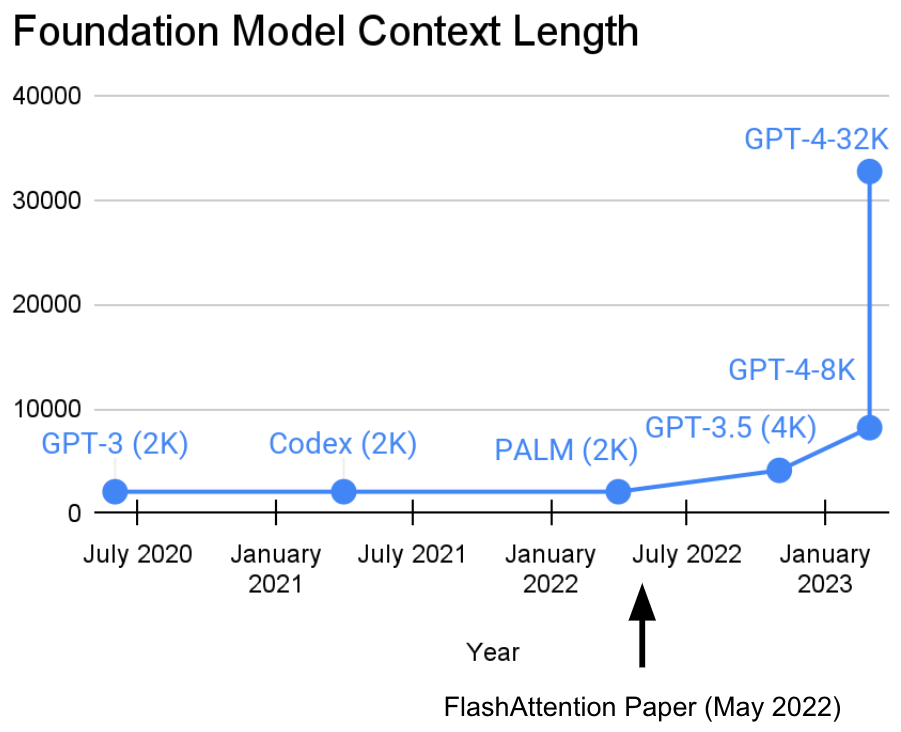
\includegraphics[width=0.75\linewidth]{figure/context.png}
    \end{figure}
\end{frame}

\begin{frame}{Issues with Transformers}

    \begin{itemize}
        \item Training: quadratic time complexity 
        \begin{itemize}
            \item Expensive for long sequence modeling (e.g., video or DNA modeling)
         \end{itemize}
        \item Inference: linear memory complexity
        \begin{itemize}
            \item Requires storing KV cache for each token
            \item High memory burden.
        \end{itemize}
    \end{itemize}    

\end{frame}

\begin{frame}{Revisiting RNNs}
    \begin{figure}
        \centering
        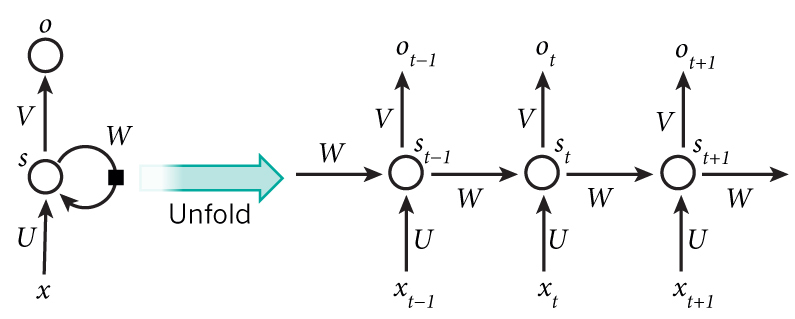
\includegraphics[width=.75\linewidth]{figure/rnn.png}
    \end{figure}
    \begin{itemize}
            \item Training: linear complexity, however, traditional RNNs are not parallelizable.
            \vspace{2mm}
            \item Inference: constant memory
    \end{itemize}
\end{frame}


\begin{frame}{Modern linear recurrent models}
    Use linear recurrence for parallel training
    \vspace{2mm}
    \begin{itemize}
        \item Gated linear RNNs (HGRN, Griffin, ...)
        \item State-space models (S4, Mamba, ...)
        \item Linear attention (RetNet, GLA, xLSTM, DeltaNet, ...)
    \end{itemize}

\end{frame}


\begin{frame}{Modern linear recurrent models}
    Use linear recurrence for parallel training
    \vspace{2mm}
    \begin{itemize}
        \item \textcolor{gray}{Gated linear RNNs (HGRN, Griffin, ...)}
        \item \textcolor{gray}{State-space models (S4, Mamba, ...)}
        \item \color{red}\textbf{Linear attention (RetNet, GLA, xLSTM, DeltaNet, ...)}
    \end{itemize}
    \vspace{2mm}
    \textcolor{black}{Linear attention is the focus of this talk.}
\end{frame}


\begin{frame}{}
    \begin{figure}
        \centering
        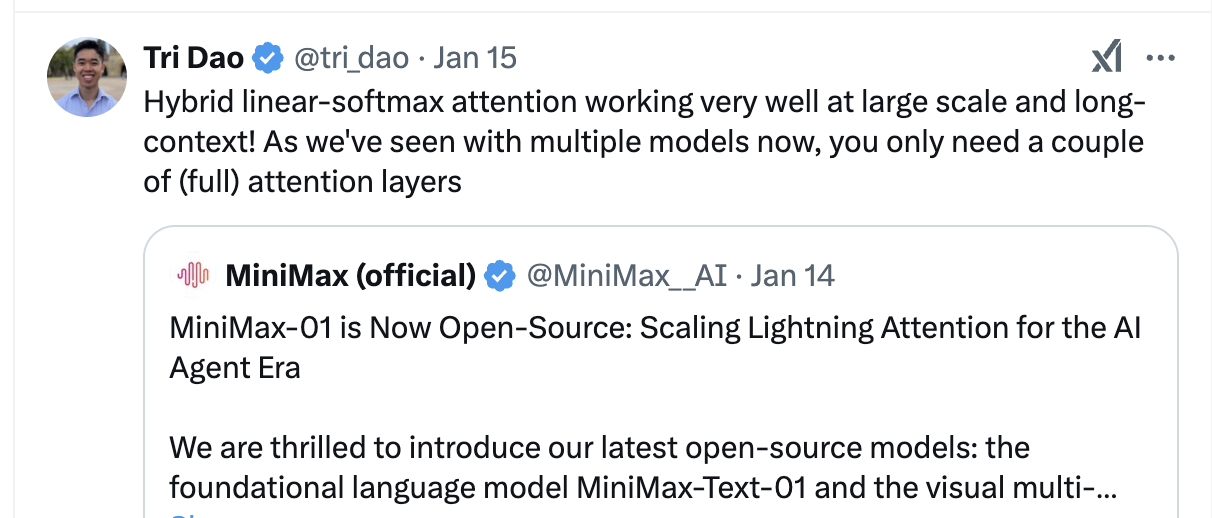
\includegraphics[width=.95\linewidth]{figure/hybrid_twitter.png}
    \end{figure}
    
    MiniMax-01 (\cite{minimax2025minimax01scalingfoundationmodels}) used hybrid attention: \textcolor{red}{\textbf{7/8}} linear attention layers + \textcolor{red}{\textbf{1/8}} softmax attention layers, with simple linear attention using data-independent decay: Lightning-Attention (\cite{Qin2024VariousLC}).
\end{frame}




\begin{frame}{}
    \centering
    \LARGE
     Linear attention  
\end{frame} 


\begin{frame}{Softmax attention}
     Attention:
    \[
    \begin{aligned}
        \mathrm{Parallel\ training:} &&& \mathbf{O} = \mathrm{softmax}(\mathbf{Q}\mathbf{K}^\top \odot \mathbf{M})\mathbf{V} &&\in \mathbb{R}^{L\times d}   \\
        \mathrm{Iterative\ inference:} &&&\mathbf{o_t} = \sum_{j=1}^t \frac{\exp(\mathbf{q}_t^\top \mathbf{k}_j)}{\sum_{l=1}^t\exp(\mathbf{q}^\top_t \mathbf{k}_l)}\mathbf{v}_j &&\in \mathbb{R}^d 
    \end{aligned}
    \]
    where $\mathbf{M} \in \mathbb{R}^{L \times L}$ is the casual mask:
    \[
    \mathbf{M}_{i,j} = \begin{cases}
        -\infty & \text{if } j > i \\
        1 & \text{if } j \leq i
    \end{cases}
    \]
\end{frame}

\begin{frame}{Linear attention = standard attention - softmax}
    Linear attention (\cite{katharopoulos2020transformers}):
    \[
    \begin{aligned}
        \mathrm{Parallel\ training:} &&& \mathbf{O} = \hcancel[red]{\mathrm{softmax}}(\mathbf{Q}\mathbf{K}^\top \odot \mathbf{M})\mathbf{V} &&\in \mathbb{R}^{L\times d}   \\
        \mathrm{Iterative\ inference:} &&&\mathbf{o_t} = \sum_{j=1}^t \frac{\hcancel[red]{\exp}(\mathbf{q}_t^\top \mathbf{k}_j)}{\hcancel[red]{\sum_{l=1}^t\exp(\mathbf{q}^\top_t \mathbf{k}_l)}}\mathbf{v}_j &&\in \mathbb{R}^d 
    \end{aligned}
    \]
    where $\mathbf{M}$ is the causal mask for linear attention:
    \[
    \mathbf{M}_{i,j} = \begin{cases}
        0 & \text{if } j > i \\
        1 & \text{if } j \leq i
    \end{cases}
    \] 
\end{frame}

\begin{frame}{Equivalent View: Matrix-Valued Hidden States}
    $$ \begin{aligned}  
        \mathbf{o_t} &=  \sum_{j=1}^t (\mathbf{q}_t^\top \mathbf{k}_j) \mathbf{v}_j \\
         &= \sum_{j=1}^t \mathbf{v}_j(\mathbf{k}_j^\top \mathbf{q}_t) &  \mathbf{k}_j^\top \mathbf{q}_t = \mathbf{q}_t^\top \mathbf{k}_j \in \mathbb{R}\\  
        &= {\color{red}\underbrace{(\sum_{j=1}^t \mathbf{v}_j\mathbf{k}_j^\top)}_{\mathbf{S}_t \in \mathbb{R}^{d \times d}}}\mathbf{q}_t & \text{By associativity}
    \end{aligned} $$    
\end{frame}

\begin{frame}{Linear attention = Linear RNN + matrix-valued hidden states}
    Let $\mathbf{S}_t = \sum_{j=1}^t\mathbf{v}_j\mathbf{k}_j^\top \in \mathbb{R}^{d \times d}$ be the matrix-valued hidden state, then:
    $$ \begin{aligned}
        \mathbf{S}_t &= \mathbf{S}_{t-1} + \mathbf{v}_t\mathbf{k}_t^\top &&\in \mathbb{R}^{d \times d}  \\
        \mathbf{o}_t &= \mathbf{S}_t\mathbf{q}_t &&\in \mathbb{R}^d  
    \end{aligned} $$
    
\begin{itemize}
    \item Linear attention implements {\color{red}\textbf{elementwise linear recurrence}}.
    \item Linear attention has a {\color{red}\textbf{matrix-valued hidden state}}, significantly increasing the state size.
\end{itemize}
\end{frame}
\begin{frame}{Challenges in training: the parallel form}
    \centering
    \begin{align*}
        \mathbf{O}= (\mathbf{Q}\mathbf{K}^\top \odot \mathbf{M})\mathbf{V} \in \mathbb{R}^{L\times d} &&
    \end{align*}
    \vspace{2mm}

    The time complexity is still quadratic in sequence length, which is problematic for long sequences.
\end{frame}

\begin{frame}{Challenges in training: the recurrent form}
    \[
    \begin{aligned}
        \mathbf{S}_t &= \mathbf{S}_{t-1} + {\color{blue}\mathbf{v}_t\mathbf{k}_t^\top} &&\in \mathbb{R}^{d \times d}  \\
        \mathbf{o}_t &= {\color{orange}\mathbf{S}_t\mathbf{q}_t} &&\in \mathbb{R}^d  
    \end{aligned}
    \]

     Poor GPU utilization due to:
        \begin{itemize}
            \item Sequential computation limits parallelization opportunities across the sequence dimension.
            \item {\color{blue}Rank-1 outer product updates} and {\color{orange}matrix-vector multiplications} are not optimized for GPU tensor cores, which are designed for dense matrix-multiply operations (typically at least 16x16 matrix sizes).
        \end{itemize}   
    
\end{frame}


\begin{frame}{Chunkwise parallel form}
    \textbf{Chunkwise Form:}
    \begin{itemize}
        \item Interpolates between recurrent and parallel forms.
        \item Splits a sequence of length $L$ into $L/C$ chunks of size $C$:
            \begin{itemize}
                \item When $C=1$, it reduces to the recurrent form.
                \item When $C=L$, it reduces to the parallel form.
            \end{itemize}
        \item  \textbf{Key Property:} Chunkwise form is {\color{red} \textbf{NOT an approximation}}—it computes the exact same output as the original formulation.
        \end{itemize}
\end{frame}

\begin{frame}{Chunkwise parallel form}
    Chunkwise form computes only the {\color{red} \textbf{last hidden state}} per chunk. 
    \\
    Output is derived from:
                \begin{itemize}
                \item {\color{red} \textbf{Recurrent Form:}} Historical context across chunks.
                \item {\color{red} \textbf{Parallel Form:}} Local context within a chunk.
            \end{itemize}
\end{frame}

\begin{frame}{Notations}
 
    \begin{align*}
        \mathbf{S}_{[i]} &:= \mathbf{S}_{iC} \in \mathbb{R}^{d \times d} &&\text{the last hidden state of chunk $i$}, \\
        \mathbf{Q}_{[i]} &= \mathbf{Q}_{iC+1:(i+1)C} \in \mathbb{R}^{C \times d} &&\text{the query block of chunk $i$}. \\
    \end{align*}
    We define $\mathbf{K}_{[i]}, \mathbf{V}_{[i]}, \mathbf{O}_{[i]}$ in a similar way.
\end{frame}

% \begin{frame}
%     \centering
%     \LARGE
%       Linear attention with decay
% \end{frame}


% \begin{frame}{Hardware-efficient training with chunkwise parallel form}
%             \begin{itemize}
%                 \item \textcolor{gray!50}{Sequence of length $L$ divided into $L/C$ chunks of size $C$}
%                 \item \textcolor{gray!50}{Compute only the {last hidden state} of each chunk.}
%                 \item \textcolor{gray!50}{Compute the output from two parts:}
%                 \begin{itemize}
%                     \item \textcolor{gray!50}{Historical context: using recurrent form}
%                     \item \textcolor{gray!50}{Local context: using parallel form}
%                 \end{itemize}
%                 \item When $C=1$, it reduces to recurrent form; when $C=L$, it reduces to parallel form.
%                 \item Chunkwise form is {\color{red} \textbf{NOT an approximation}}, it computes the exact same output.
%             \end{itemize}
    
%             \vspace{2mm}
%             Notation:
%             \begin{align*}
%                 \mathbf{S}_{[i]} &:= \mathbf{S}_{iC} \in \mathbb{R}^{d \times d} &&\text{(Chunk-level hidden state)} \\
%                 \square_{[i]} &= \square_{iC+1:(i+1)C} \in \mathbb{R}^{C \times d} &&\text{(Matrix block for chunk $i$)} \\
%                 &\text{for } \square \in \{\mathbf{Q}, \mathbf{K}, \mathbf{V}, \mathbf{O}\} \\
%             \end{align*}
% \end{frame}



\begin{frame}{}
    % \begin{figure}
    %     \centering
    %     \includegraphics[width=.9\linewidth]{chunk-state.png}
    % \end{figure}
    \definecolor{yellowgreen}{RGB}{154,205,50}    
\definecolor{limeyellow}{RGB}{185,215,40}     
\definecolor{yellowgreenyellow}{RGB}{173,255,47}    

\begin{tikzpicture}
    \foreach \x in {0,5,10,15} {
        \draw[dashed] (\x,-2) -- (\x,2);
    }

        \begin{scope}[shift={(-1.5,0)}]
            \node[draw=black, minimum size=1cm] (grid-0-3) at (0.5,0.5) {};
            \foreach \x in {0,0.33,0.66} {
                \foreach \y in {0,0.33,0.66} {
                    \draw[black] (\x+0.17,\y+0.17) circle (0.12);
                }
            }
        \end{scope}

    \foreach \section [count=\i] in {0.5,5.5} {
        \foreach \offset [count=\j] in {0,1.5} {
            \begin{scope}[shift={(\section+\offset,0)}]
                \node[draw=gray!50, minimum size=1cm] (grid-\i-\j) at (0.5,0.5) {};
                \foreach \x in {0,0.33,0.66} {
                    \foreach \y in {0,0.33,0.66} {
                        \draw[gray!50] (\x+0.17,\y+0.17) circle (0.12);
                    }
                }
            \end{scope}
        }
        
        \begin{scope}[shift={(\section+3,0)}]
            \node[draw=black, minimum size=1cm] (grid-\i-3) at (0.5,0.5) {};
            \foreach \x in {0,0.33,0.66} {
                \foreach \y in {0,0.33,0.66} {
                    \draw[black] (\x+0.17,\y+0.17) circle (0.12);
                }
            }
        \end{scope}
    }
    
    \foreach \section [count=\i] in {0.5,5.5} {
        \begin{scope}[shift={(\section,-1.5)}]
            \foreach \offset [count=\j] in {0,1.5,3} {
                \node[fill=blue!20,draw=black, minimum width=1cm, minimum height=0.4cm] (rect-\i-\j) at (\offset+0.5,0.2) {};
                \foreach \x in {0.2, 0.5, 0.8} {
                    \draw[black] (\offset+\x,0.2) circle (0.1);
                }
                \draw[->,red!30,very thick] (rect-\i-\j.north) to[out=90,in=-90, looseness=0.7] 
                    ([xshift=\j*0cm]grid-\i-3.south);
            }
        \end{scope}
    }
    
% \draw[->,yellowgreen,very thick] (grid-1-3.east) to[bend left=60] node[above,font=\small,xshift=-0.5cm]{$\color{black}\boldsymbol{S}_{[2]}=\boldsymbol{S}_{[1]}{\color{yellowgreen}(\boldsymbol{I}-\boldsymbol{W}_{[2]}^\top \boldsymbol{K}_{[2]})} + {\color{red}\boldsymbol{U}_{[2]}^\top \boldsymbol{K}_{[2]}}$}  (grid-2-3.west);
\draw[->,black, thick] (grid-0-3.east)  to[bend left=60] (grid-1-3.west);
\draw[->,black, thick] (grid-1-3.east)  to[bend left=60] 
node[above,xshift=-1.5cm, yshift=0.5cm,align=center]{
  \textcolor{black}{{\large{\textbf{\color{red}Sequential}} Chunk-Level State Passing:}} \\
%   $\color{black}\boldsymbol{S}_{[i+1]}=\boldsymbol{S}_{[i]}
% + 
%     {\color{blue!50}\colorbox{red!30}{$\boldsymbol{V}_{[i]}^\top \boldsymbol{K}_{[i]}$}}$
} (grid-2-3.west);


\end{tikzpicture}

    \begin{align*}
        &\mathbf{S}_{[t+1]} = \underbrace{\mathbf{S}_{[t]}}_{\mathbb{R}^{d\times d}} + \colorbox{red!30}{$\underbrace{\color{blue!50}\mathbf{V}_{[t]}^\top}_{\mathbb{R}^{d\times C}} \underbrace{\color{blue!50}\mathbf{K}_{[t]}}_{\mathbb{R}^{C\times d}}$} &&\in \mathbb{R}^{d\times d}  \\
    \end{align*}
    Computational Complexity: $\mathcal{O}(Cd^2)$ per chunk and $\mathcal{O}(Ld^2)$ for the entire sequence.
\end{frame}

\begin{frame}{}
    
\begin{tikzpicture}[
    box/.style={
        rectangle,
        minimum size=0.5cm,
        draw=black!20
    }
]
    \foreach \x in {0,5,10,15} {
        \draw[dashed] (\x,-2) -- (\x,2);
    }
            \begin{scope}[shift={(-1.5,0)}]
            \node[draw=black, minimum size=1cm] (grid-0-3) at (0.5,0.5) {};
            \foreach \x in {0,0.33,0.66} {
                \foreach \y in {0,0.33,0.66} {
                    \draw[black] (\x+0.17,\y+0.17) circle (0.12);
                }
            }
        \end{scope}


    \foreach \section [count=\i] in {0.5,5.5} {

        % \foreach \offset [count=\j] in {0,1.5} {

     \begin{scope}[shift={(\section+1.5,0.1)}]

        \node[box, fill=red!100, minimum size=0.33cm] at (0.17,0.83) {};
        \node[box, minimum size=0.33cm] at (0.5,0.83) {};
        \node[box, minimum size=0.33cm] at (0.83,0.83) {};
        
        \node[box, fill=red!15, minimum size=0.33cm] at (0.17,0.5) {};
        \node[box, fill=red!75, minimum size=0.33cm] at (0.5,0.5) {};
        \node[box, minimum size=0.33cm] at (0.83,0.5) {};
        

        \node[box, fill=red!25, minimum size=0.33cm] at (0.17,0.17) {};
        \node[box, fill=red!45, minimum size=0.33cm] (attn-\i)at (0.5,0.17) {};
        \node[box, fill=red!65, minimum size=0.33cm] at (0.83,0.17) {};
    \end{scope}

        \begin{scope}[shift={(\section+3,0)}]
            \node[draw=black, minimum size=1cm] (grid-\i-3) at (0.5,0.5) {};
            \foreach \x in {0,0.33,0.66} {
                \foreach \y in {0,0.33,0.66} {
                    \draw[black] (\x+0.17,\y+0.17) circle (0.12);
                }
            }
        \end{scope}
    }
    

    \foreach \section [count=\i] in {0.5,5.5} {
        \begin{scope}[shift={(\section,-1.5)}]

            \foreach \offset [count=\j] in {0,1.5,3} {
                \node[draw=black, fill=blue!20, minimum width=1cm, minimum height=0.4cm] (rect-\i-\j) at (\offset+0.5,0.2) {};

                \foreach \x in {0.2, 0.5, 0.8} {
                    \draw[black] (\offset+\x,0.2) circle (0.1);
                }
                \node[draw=black, minimum width=1cm, minimum height=0.4cm,fill=orange!30] (upper-rect-\i-\j) at (\offset+0.5,0.2+3.5) {};
                \foreach \x in {0.2, 0.5, 0.8} {
                    \draw[black] (\offset+\x,0.2+3.5) circle (0.1);
                }
                
            
    \pgfmathsetmacro{\prevsection}{\i-1}
\draw[->, yellowgreen, thick] 
    (grid-\the\numexpr\i-1\relax-3.east) 
    to[bend left=20] 
    (upper-rect-\i-\j.west);

\draw[->, yellowgreen, thick] 
    (rect-\i-\j.north) 
    to[bend left=30] 
    (upper-rect-\i-\j.west);

\draw[->,red!50,very thick] (rect-\i-\j.north) to[out=90,in=-90,looseness=1.2] (attn-\i.south);

\draw[->,red!50,very thick] ([yshift=0.6cm]attn-\i.north) to[out=90,in=-90,looseness=1.2] (upper-rect-\i-\j.south);

}

\ifnum\i>1
\fi

        \end{scope}
    }
    
\node[above=0.25cm,xshift=-3cm,align=center] at (upper-rect-2-2.north) {
  \textcolor{black}{\large{\textbf{\color{red}Parallel} Output Computation:}} \\
%   ${\color{orange}\mathbf{O}_{[i]}}=\colorbox{yellowgreen!30}{${\color{blue!50}\mathbf{Q}_{[i]}}\mathbf{S}_{[i]}^\top$}+\colorbox{red!30}{\color{blue!50}$\left({\mathbf{Q}_{[i]}\mathbf{K}_{[i]}^\top \odot \mathbf{M}}\right)\mathbf{V}_{[i]}$}$
};

\end{tikzpicture}

    \vspace{-3mm}
    \begin{align*}
        {\color{orange}\mathbf{O}_{[t]}} = \colorbox{yellowgreen!30}{$\underbrace{{\color{blue!50}\mathbf{Q}_{[t]}}\mathbf{S}_{[t]}^\top}_{\text{inter-chunk}:\mathbf{O}_{[t]}^{\text{inter}}}$} + \colorbox{red!30}{$\underbrace{({\color{blue!50}\mathbf{Q}_{[t]}\mathbf{K}_{[t]}^\top \odot \mathbf{M}}){\color{blue!50}\mathbf{V}_{[t]}}}_{\text{intra-chunk}:\mathbf{O}_{[t]}^{\text{intra}}}$} \in \mathbb{R}^{C\times d}
    \end{align*}

    Computational Complexity: $\mathcal{O}(C^2d+Cd^2)$ per chunk. $\mathcal{O}(Ld^2+LCd)$ for the entire sequence.
\end{frame}
\begin{frame}{Chunkwise parallel form}
    \begin{itemize}
        \item {\textcolor{black}{Total complexity}}: $\mathcal{O}(Ld^2 + LdC)$, achieving {\textcolor{red}{subquadratic complexity}} in sequence length when $C$ is small.
        \item {\textcolor{black}{Practical settings}}: $C$ is typically set to $\{64, 128, 256\}$.
        \item {\textcolor{black}{Extensibility}}: Can be generalized to linear attention with {\textcolor{red}{decay or delta rule}} (to be discussed later).
        \item {\textcolor{black}{Adoption}}: The {\color{red}de facto standard} for {\color{red}training modern linear attention models}, including:
        \begin{itemize}
            \item {\textcolor{black}{Mamba2}}, {\textcolor{black}{Based}}, {\textcolor{black}{GLA}}, {\textcolor{black}{DeltaNet}}, {\textcolor{black}{Lightning Attention}}, {\textcolor{black}{mLSTM}}, and others.
        \end{itemize}
    \end{itemize}
\end{frame}

\begin{frame}{Flash linear attention}
    \begin{figure}
        \centering
        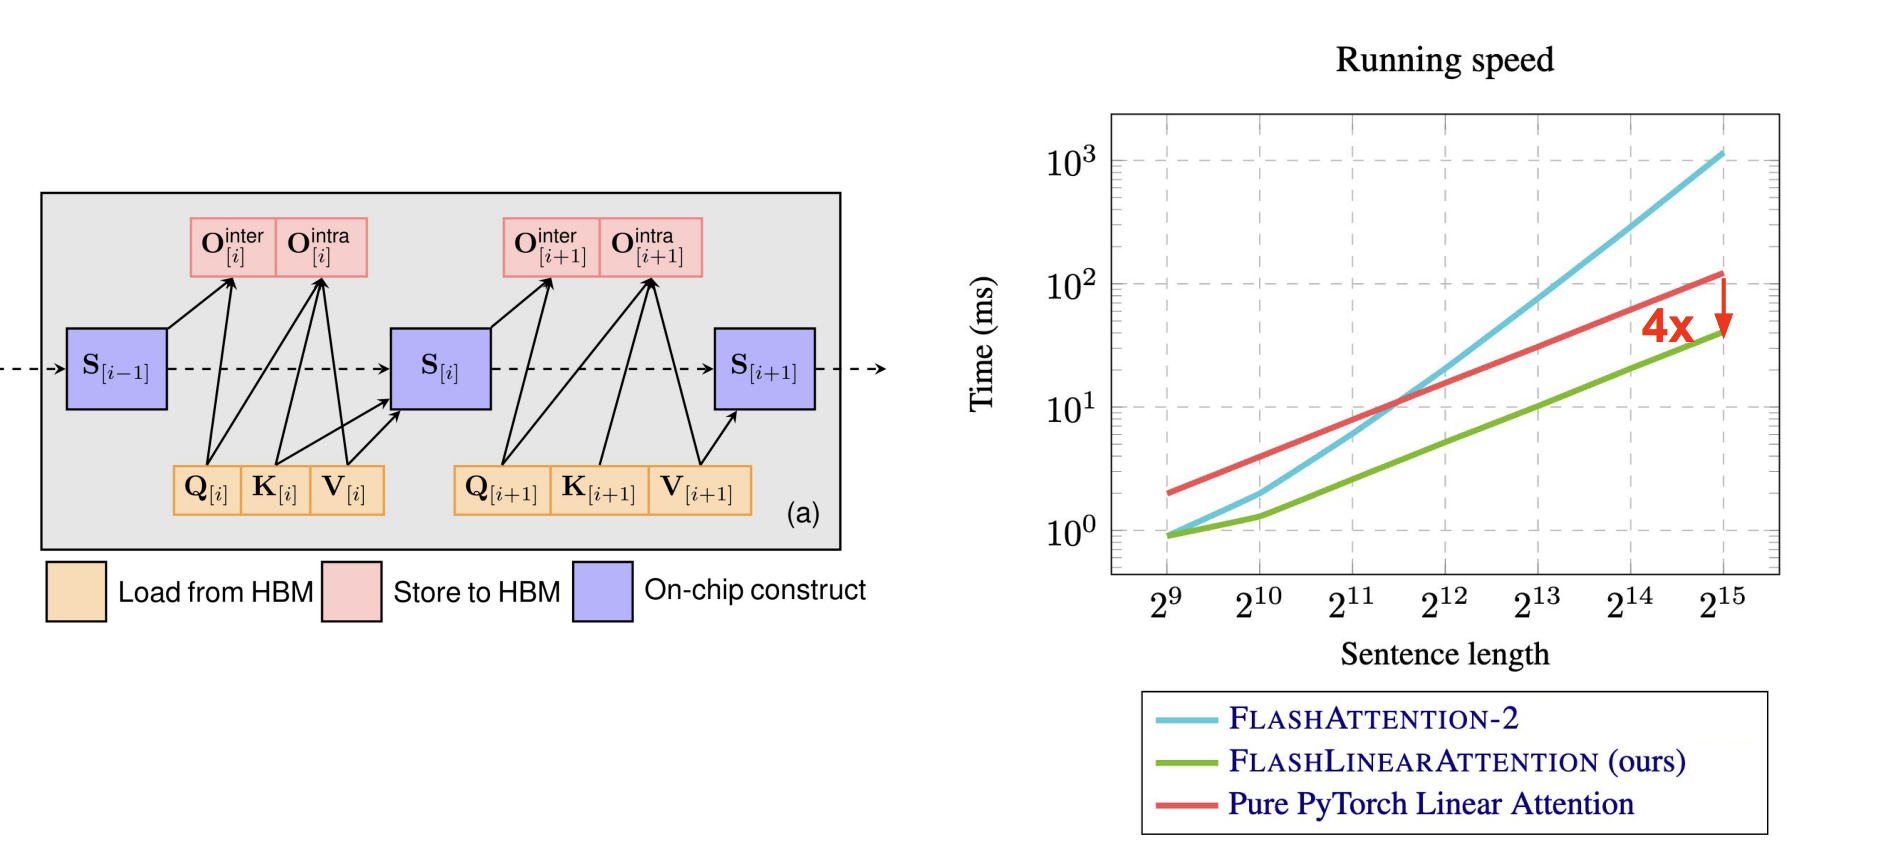
\includegraphics[width=.9\linewidth]{figure/fla-speed.png}
    \end{figure}
    \vspace{2mm} 
    I/O optimization significantly improves the wall-clock time.
\end{frame}

\begin{frame}{Flash linear attention}
    \begin{figure}
        \centering
        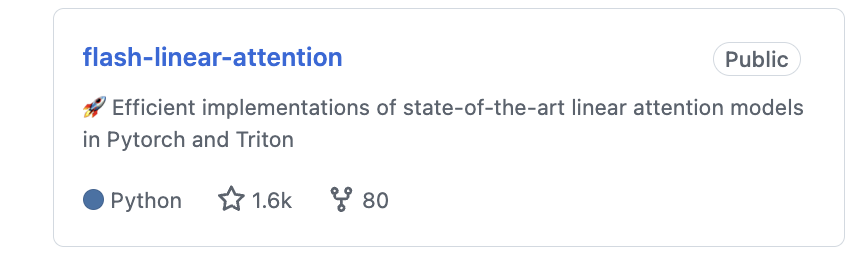
\includegraphics[width=.9\linewidth]{figure/fla-repo.png}
    \end{figure}
    The Flash Linear Attention library provides hardware-efficient implementation of various linear attention models.
    \begin{itemize}
        \item RetNet, GLA, Based, HGRN2, RWKV6, GSA, Mamba2, DeltaNet, Gated DeltaNet, RWKV7  ...
    \end{itemize}
\end{frame}

\begin{frame}{Summary}
    \begin{itemize}
        \item Linear attention = Softmax attention - softmax.
        \item Linear attention = Linear RNN + {\color{red}{matrix-valued hidden state}}.
        \item The chunkwise parallel form is more {\color{red}{hardware-friendly}} than the recurrent and parallel forms.
        \item Flash Linear Attention is an {\color{red}{I/O-aware}} implementation of the chunkwise parallel form.
    \end{itemize}
\end{frame}

\begin{frame}{}
    \centering
    \LARGE
     Linear attention with decay
\end{frame} 



\begin{frame}{Linear attention is not enough}
    \begin{align*}
        \mathbf{S}_t &= \mathbf{S}_{t-1} + \mathbf{v}_t\mathbf{k}_t^\top &&\in \mathbb{R}^{d \times d}  \\
        \mathbf{o}_t &= \mathbf{S}_t\mathbf{q}_t &&\in \mathbb{R}^d  
    \end{align*}
    \vspace{3mm}
    Vanilla linear attention {\color{red}performs poorly in language modeling}.
    \begin{itemize}
        \item Only stores key-value pairs in memory.
        \item Has no mechanism to forget old memories.
        \item Leads to memory saturation and degradation in performance since the memory size is fixed.
    \end{itemize}
\end{frame}


\begin{frame}{Linear attention with data-independent decay}
    \begin{align*}
        \mathbf{S}_t &= {\color{red}\gamma} \mathbf{S}_{t-1} + \mathbf{v}_t\mathbf{k}_t^\top &&\in \mathbb{R}^{d \times d}  \\
        \mathbf{o}_t &= \mathbf{S}_t\mathbf{q}_t &&\in \mathbb{R}^d  
    \end{align*}
    \begin{itemize}
        \item ${\color{red}\gamma}$ is a constant exponential decay factor ${\color{red}0 < \gamma < 1}$.
        \item This mechanism {\color{red}weighs recent tokens more than distant tokens}, and language modeling has a strong {\color{red}recency bias}.
        \item Works well in practice: RetNet (\cite{sun2023retentive}), Lightning Attention (\cite{Qin2024VariousLC}).
    \end{itemize}
\end{frame}


\begin{frame}{Linear attention with data-dependent decay}
    \begin{align*}
        \mathbf{S}_t &= {\color{red}\gamma_t} \mathbf{S}_{t-1} + \mathbf{v}_t\mathbf{k}_t^\top &&\in \mathbb{R}^{d \times d}  \\
        \mathbf{o}_t &= \mathbf{S}_t\mathbf{q}_t &&\in \mathbb{R}^d  
    \end{align*}
    \begin{itemize}
        \item ${\color{red}{\gamma_t} \in (0, 1)}$ is a data-dependent decay term that is a function of $\mathbf{x}_t$.
        \item Enables dynamic control of memory retention/forgetting based on input data.
        \item Examples: Mamba2 (\cite{mamba2}), mLSTM (\cite{beck2024xlstm}), Gated Retention (\cite{sun2024you}).
    \end{itemize}
\end{frame}

\begin{frame}{The parallel form for linear attention with decay}
    \begin{align*}
        \mathbf{S}_t &= {\color{red}\gamma_t} \mathbf{S}_{t-1} + \mathbf{v}_t\mathbf{k}_t^\top &&\in \mathbb{R}^{d \times d}  \\
        \mathbf{o}_t &= \mathbf{S}_t\mathbf{q}_t &&\in \mathbb{R}^d  
    \end{align*}

    Linear attention with decay has the following parallel form:
    \begin{align*}
        \mathbf{O} &= (\mathbf{Q}\mathbf{K}^\top \odot {\color{red} \mathbf{D}})\mathbf{V} \in \mathbb{R}^{L\times d} && \\
        \color{red} \mathbf{D}_{i,j} &= \begin{cases}
            \prod_{m=j+1}^i {\color{red}\gamma_m} & \text{if } i > j \\
            1 & \text{if } i = j \\
            0 & \text{otherwise}
        \end{cases}
    \end{align*}

     The duality between recurrent and parallel forms is referred to as {\color{red} state space duality (SSD)} in Mamba2 (\cite{mamba2}).
\end{frame}

% \begin{frame}{The chunkwise parallel form for linear attention with decay}
%     \begin{align*}
%         \mathbf{S}_t &= {\color{red}\gamma_t} \mathbf{S}_{t-1} + \mathbf{v}_t\mathbf{k}_t^\top &&\in \mathbb{R}^{d \times d} &&& \mathbf{o}_t &= \mathbf{S}_t\mathbf{q}_t &&\in \mathbb{R}^d 
%     \end{align*}
%     Linear attention with decay has the following chunkwise form:
%     \begin{align*}
%         \mathbf{S}_{[t]} &= {\color{red}\beta_{tC}} \mathbf{S}_{[t-1]}  +  (\mathbf{V}_{[t]} \odot {\color{red}\frac{\beta_{tC}}{\beta_{[t]}}[:,\, \text{None}]})^\top \mathbf{K}_{[t]} &&\in \mathbb{R}^{d \times d}  \\
%         \mathbf{O}_{[t]} &= \underbrace{(\mathbf{Q}_{[t]} \mathbf{S}_{[t]}^\top) \odot {\color{red}\beta_{[t]}[:,\, \text{None}]}}_{\text{inter-chunk}} + \underbrace{(\mathbf{Q}_{[t]} \mathbf{K}_{[t]}^\top \odot {\color{red}\mathbf{D}_{[t]}}) \mathbf{V}_{[t]}}_{\text{intra-chunk}} &&\in \mathbb{R}^{C \times d} 
%     \end{align*}
%     The chunkwise form with decay is {\color{blue}\textbf{mathematically equivalent}} to Mamba2's {\color{red}\textbf{SSD block decomposition algorithm}}.
% \end{frame}

% \begin{frame}{The chunkwise parallel form for linear attention with decay}
%     \begin{align*}
%         \mathbf{S}_{[t]} &= {\color{red}\beta_{tC}} \mathbf{S}_{[t-1]}  +  (\mathbf{V}_{[t]} \odot {\color{red}\frac{\beta_{tC}}{\beta_{[t]}}[:,\, \text{None}]})^\top \mathbf{K}_{[t]} &&\in \mathbb{R}^{d \times d}  \\
%         \mathbf{O}_{[t]} &= \underbrace{(\mathbf{Q}_{[t]} \mathbf{S}_{[t]}^\top) \odot {\color{red}\beta_{[t]}[:,\, \text{None}]}}_{\text{inter-chunk}} + \underbrace{(\mathbf{Q}_{[t]} \mathbf{K}_{[t]}^\top \odot {\color{red}\mathbf{D}_{[t]}}) \mathbf{V}_{[t]}}_{\text{intra-chunk}} &&\in \mathbb{R}^{C \times d} 
%     \end{align*}
%     \begin{itemize}
%         \item<1-1> $\mathbf{S}_{[t]}:=\mathbf{S}_{tC} \in \mathbb{R}^{d \times d}$. $\square_{[t]}:=\square_{tC+1:(t+1)C} \in \mathbb{R}^{C \times d}$ for $\square \in \{\mathbf{Q}, \mathbf{K}, \mathbf{V}, \mathbf{O}\}$.
%         \item<1-1> ${\color{red} \beta_{[t]} \in \mathbb{R}^{C}}$ represents the cumulative decay values within chunk $t$, where the $i$-th element is ${\color{red}(\beta_{[t]})_i= \beta_{tC+i}= \prod_{m=tC+1}^{tC+i}\gamma_m \in \mathbb{R}}$
%         \item<1-1> ${\color{red}(\mathbf{D}_{[t]})_{i,j}} = \begin{cases}
%             {\color{red}\prod_{m=tC+i+1}^{tC+j} \gamma_m} & \text{if } i < j \\
%             1 & \text{if } i = j \\
%             0 & \text{otherwise}  
%         \end{cases} \qquad \in \mathbb{R}^{C \times C}$ 
%     \end{itemize}

%     We highlight the decay-related terms in red and if we remove these red terms, we recover the chunkwise form of vanilla linear attention.

% \end{frame}



% \begin{frame}{The chunkwise parallel form for linear attention with decay}
%     \begin{align*}
%         \mathbf{S}_t &= {\color{red}\gamma_t} \mathbf{S}_{t-1} + \mathbf{v}_t\mathbf{k}_t^\top &&\in \mathbb{R}^{d \times d} &&& \mathbf{o}_t &= \mathbf{S}_t\mathbf{q}_t &&\in \mathbb{R}^d 
%     \end{align*}
%     Linear attention with decay has the following chunkwise form:
%     \begin{align*}
%         \mathbf{S}_{[t]} &= {\color{red}\beta_{Ct}} \mathbf{S}_{[t-1]}  +  (\mathbf{V}_{[t]} \odot {\color{red}\frac{\beta_{tC}}{\beta_{[t]}}[:,\, \text{None}]})^\top \mathbf{K}_{[t]} &&\in \mathbb{R}^{d \times d}  \\
%         \mathbf{O}_{[t]} &= \underbrace{(\mathbf{Q}_{[t]} \mathbf{S}_{[t]}^\top) \odot {\color{red}\beta_{[t]}[:,\, \text{None}]}}_{\text{inter-chunk}} + \underbrace{(\mathbf{Q}_{[t]} \mathbf{K}_{[t]}^\top \odot {\color{red}\mathbf{D}_{[t]}}) \mathbf{V}_{[t]}}_{\text{intra-chunk}} &&\in \mathbb{R}^{C \times d} 
%     \end{align*}
%     \begin{itemize}
%         \item Preserves matrix-multiply structure with minimal overhead when incorporating decay
%         \item As fast as vanilla linear attention's chunkwise form
%         \item Equivalent to Mamba2's block decomposition-based {\color{red} \textbf{SSD algorithm}} (\cite{mamba2}).
%     \end{itemize}

% \end{frame}






\begin{frame}{Linear attention with more fine-grained decay}

    \begin{align*}
        \mathbf{S}_t &= {\color{red}\mathbf{G}_t} \odot \mathbf{S}_{t-1} + \mathbf{v}_t\mathbf{k}_t^\top &&\in \mathbb{R}^{d \times d}  \\
        \mathbf{o}_t &= \mathbf{S}_t\mathbf{q}_t &&\in \mathbb{R}^d  
    \end{align*}
    % where {\color{red}$\mathbf{G}_t \in \mathbb{R}^{d \times d}$} is a data-dependent gate matrix. 

    \textbf{Condition} for the matmul-based (chunkwise) parallel form (\cite{gla}):
    \[{\color{red}\mathbf{G}_t = \boldsymbol{\beta}_t\boldsymbol{\alpha}_t^\top \in \mathbb{R}^{d\times d}, \quad \boldsymbol{\alpha}_t, \boldsymbol{\beta}_t \in \mathbb{R}^d}
    \]

    \begin{itemize}
        \item Mamba-1 (\cite{Gu2023MambaLS}) does not conform to this structure, preventing the use of tensor cores.
        \item It is common to set ${\color{red}\boldsymbol{\beta}_t = \mathbf{1}}$ in practice, examples: GLA (\cite{gla}), RWKV6 (\cite{rwkv6}), GSA (\cite{zhang2024gated}), HGRN2 (\cite{hgrn2}).
    \end{itemize}

\end{frame}

\begin{frame}{Summary}
    \begin{itemize}
        \item Language modeling has a strong {\color{red}recency bias}.
        \item Decay helps {\color{red}bridge the perplexity gap} between linear and softmax attention.
        \item {\color{red}Fine-grained decay} enhances performance but poses scaling challenges.
        \item {\color{red}Outer-product structure} enables efficient chunkwise training with fine-grained decay.
    \end{itemize}
\end{frame}



\begin{frame}{}
    \centering
    \LARGE
    Toward more expressive update rule: \\the delta rule
\end{frame}

\begin{frame}{Linear attention is secretly a fast weight programmer}
\[
    \mathbf{o}_t = \mathbf{S}_t \mathbf{q}_t
\]
We can think of the recurrent hidden state $\mathbf{S}_t$ as a fast weight matrix that maps input $\mathbf{q}_t$ to output $\mathbf{o}_t$ and is updated as it goes:
\[\mathbf{S}_t = \mathbf{S}_{t-1} + \mathbf{v}_t\mathbf{k}_t^\top\]

\end{frame}


% \begin{frame}{Gated Linear Attention: Motivation}
%     \[
%         \begin{aligned}
%             \mathbf{S}_t &= \mathbf{S}_{t-1} + \mathbf{v}_t\mathbf{k}_t^\top &&\in \mathbb{R}^{d \times d}  \\
%             \mathbf{o}_t &= \mathbf{S}_t\mathbf{q}_t &&\in \mathbb{R}^d  
%         \end{aligned}
%         \]    
% \begin{itemize}
%     \item<1-> The cumulative sum tend to explode the hidden state, leading to unstable training and poor language modeling performance.
%     \item<2-> RetNet uses data-independent decay, narrowing down the performance gap, but still underperforming Transformers.
%     \item<3-> Forget gate has been the `missing piece' in linear attention.
% \end{itemize}
% \end{frame}

% \begin{frame}{Gated Linear Attention: Full Form}
%     \begin{align*}
%         \mathbf{S}_t = \mathbf{G}_t \odot \mathbf{S}_{t-1} + \mathbf{v}_t \mathbf{k}_t^\top
%     \end{align*}
%     where $\mathbf{G}_t = \boldsymbol{\beta_t}\boldsymbol{\alpha_t}^\top$ is the gate matrix.
% \begin{itemize}
%     \item Both input $\mathbf{v}_t \mathbf{k}_t^\top$ and gate matrix $\mathbf{G}_t$ are in outer product form
%     \item This structure enables efficient computation via matrix multiplication
% \end{itemize}
% \end{frame}

% \begin{frame}{Gated Linear Attention: Simplified Form}
    
%     When $G_t = \mathbf{1} \boldsymbol{\alpha_t}^\top$:

%     \begin{align*}
%       \mathbf{O}_t =   ((\mathbf{Q} \odot \mathbf{A}) (\mathbf{K} \odot \mathbf{A}^{-1}) \odot \mathbf{M}) \mathbf{V}
%     \end{align*}
%     where $\mathbf{A}_t = \bigodot_{i=1}^t \alpha_i $ is the cumulative product of decay, and $\mathbf{A}^{-1}$ denotes element-wise inverse (not matrix inverse).
% \\
% \vspace{2mm}
% Balanced between training efficiency and expressiveness. Examples:
% \begin{itemize}
%     \item  GLA (\cite{gla})
%     \item  HGRN2 (\cite{hgrn2})
%     \item  RWKV6 (\cite{rwkv6})
%     \item  GSA (\cite{zhang2024gated})
%     \item  MetaLA (\cite{meta_la})
%     \item  ...
% \end{itemize}


% \end{frame}

% \begin{frame}{Gated Linear Attention: Simplest Form}
%     When $G_t = \alpha_t \mathbf{1} \mathbf{1}^\top$:
%     \begin{align*}
%         \mathbf{O}_t &= \left(\mathbf{Q} \mathbf{K}^\top \odot \mathbf{D} \right)\mathbf{V}, \\
%         \mathbf{D}_{ij} &= \begin{cases}
%             \prod_{k=j+1}^{i} \alpha_k & \text{if } i \geq j \\
%             0 & \text{otherwise}
%         \end{cases}
%     \end{align*}
%     Maximum training efficiency, but limited expressiveness. Examples:
%     \begin{itemize}
%         \item Mamba2 (\cite{mamba2})
%         \item xLSTM (\cite{beck2024xlstm})
%         \item Gated RetNet (\cite{Sun2024YouOC})
%     \end{itemize}


% \end{frame}



\begin{frame}{Linear attention as a fast weight programming perspective}
    \resizebox{\linewidth}{!}{
    \begin{tikzpicture}[
        node distance=4.5cm,
        box/.style={
            rectangle,
            draw,
            minimum height=1cm,
            minimum width=1.2cm,
            thick,
            fill=blue!10
        },
        arrow/.style={->,>=latex,thick},
        small box/.style={
            rectangle,
            draw,
            minimum width=0.8cm,
            minimum height=0.8cm,
            inner sep=2pt,
            font=\sffamily,
            fill=orange!10
        },
        values box/.style={
            rectangle,
            draw,
            pattern=north west lines,
            pattern color=green!40,
            fill=green!10,
            minimum size=0.8cm,
            thick
        },
        pink box/.style={
            rectangle,
            draw=pink!80!red,
            thick,
            minimum height=1.2cm,
            minimum width=3cm,
            fill=pink!20,
        },
        weight box/.style={
            rectangle,
            draw=blue!60,
            thick,
            minimum height=1cm,
            minimum width=8cm,
            align=center,
            fill=blue!5
        },
        fast weight box/.style={
            rectangle,
            draw=orange,
            thick,
            fill=orange,
            fill opacity=0.3,
            draw opacity=0.5,
            text opacity=1
        }
    ]
    
    \begin{scope}[on background layer]
        % 状态框
        \node (M1) at (3, 0) {};
        \node[box] (M2) at (4.5,0) {$\mathbf{S}_{t-1}$};
        \node[box] (M3) at (9,0) {$\mathbf{S}_{t}$};
        \node[box] (M4) at (13.5,0) {$\mathbf{S}_{i+1}$};
        
        % Fast weights包裹框
        \path (2.5, 0) -- (M4.south east) node[midway,yshift=-0.5cm] (note) {\small\textbf{\textcolor{orange}{(rapidly changes at each time step)}}};
        \node[fast weight box,fit=(M1)(M2)(M3)(M4)(note),inner sep=10pt] (fastbox) {};
    \end{scope}
    
    % 输入层
    \node[left] at (0.6,6) {\sffamily\Large\bfseries inputs}; 
    \node[box] (X1) at (4.5,6) {$\mathbf{x}_{t-1}$};
    \node[box] (X2) at (9,6) {$\mathbf{x}_t$};
    \node[box] (X3) at (13.5,6) {$\mathbf{x}_{t+1}$};
    
    % Slow weights层
    \node[left] at (0.6,4) {\sffamily\Large\bfseries slow weights};
    \node[weight box] (W) at (9,4) {$\mathbf{W}_q, \mathbf{W}_k, \mathbf{W}_v$\\\small(shared across time steps)};
    
    % 状态间连接
    \draw[arrow] (1.5,0) -- (M2) coordinate[pos=0.95] (M12);
    \draw[arrow] (M2) -- (M3) coordinate[pos=0.95] (M23);
    \draw[arrow] (M3) -- (M4) coordinate[pos=0.95] (M34);
    \draw[arrow] (M4) -- (15.5,0) coordinate[pos=0.95];
    
    % KVQ组
    \foreach \x/\pos/\endpoint/\i/\m in {4.5/a/M12/{t-1}/M2,9/b/M23/t/M3,13.5/c/M34/{t+1}/M4} {
        \node[pink box] (PB\pos) at (\x,2) {};
        \node[small box] (K\pos) at ($(\x,2)+(-0.8,0)$) {$\mathbf{k}_{\i}$};
        \node[small box] (V\pos) at (\x,2) {$\mathbf{v}_{\i}$};
        \node[small box] (Q\pos) at ($(\x,2)+(0.8,0)$) {$\mathbf{q}_{\i}$};
        
        \draw[->,thick] (K\pos.south) to[bend right=45] (\endpoint);
        \draw[->,thick] (V\pos.south) to[bend right=25] (\endpoint);
        \draw[->,thick] (Q\pos.south) to[out=-90,in=90] (\m.north);
    }
    
    % 输入到权重的连接
    \foreach \x in {4.5,9,13.5} {
        \node (X) at (\x,6) {};
        \node (PB) at (\x,2) {};
        \draw[->,thick,blue!60] (X) to[out=-60,in=90] (W);
        \draw[->,thick,blue!60] (W) to[out=-90,in=90] (PB);
    }
    
    % 输出层
    \node[values box] (V2) at (4.5,-2.2) {$\mathbf{o}_{t-1}$};
    \node[values box] (V3) at (9,-2.2) {$\mathbf{o}_{t}$};
    \node[values box] (V4) at (13.5,-2.2) {$\mathbf{o}_{t+1}$};
    
    % 标签
    \node[left] at (0.6,2) {\sffamily\Large\bfseries queries/keys/values};
    \node[left] at (0.6,-2.2) {\sffamily\Large\bfseries outputs};
    \node[left] at (0.6,0) {\sffamily\Large\bfseries fast weights};
    
    % 输出连接
    \draw[arrow] (M2) -- (V2);
    \draw[arrow] (M3) -- (V3);
    \draw[arrow] (M4) -- (V4);
    
    \end{tikzpicture}
    
    }
        
    % - Implements a form of working memory    
%     The hidden state matrix $\mathbf{S}_t$ is a fast weight matrix that is updated at each timestep:
%     \begin{align*}
%         \mathbf{S}_t &= \mathbf{S}_{t-1} + \mathbf{v}_t \mathbf{k}_t^\top
%     \end{align*}
%     \vspace{2mm}
    
%     The fast weight matrix is used to map inputs $\mathbf{q}_t$ into outputs $\mathbf{o}_t$:
% \begin{align*}
%     \mathbf{o}_t = \mathbf{S}_t \mathbf{q}_t
\vspace{-4mm}
\begin{itemize}
    \item {\color{red}\textbf{Fast Weight}}: $\mathbf{S}_t$ maps $\mathbf{q}_t$ to $\mathbf{o}_t$, updated dynamically during inference  for rapid adaptation.
    \item {\color{red}\textbf{Slow Weight}}: $\mathbf{W}_q$, $\mathbf{W}_k$, and $\mathbf{W}_v$ are fixed during inference and only updated during training (e.g., via gradient descent).
\end{itemize}


% \begin{quote}
%     ``Fast weights provide a neurally plausible way of implementing the type of temporary storage that is required by working memory, while slow weights capture more permanent associations learned over many experiences.''
%     \small{ -- Geoffrey Hinton}
% \end{quote}


\end{frame}

\begin{frame}{The choice of update rule}
    \begin{figure}
        \centering
        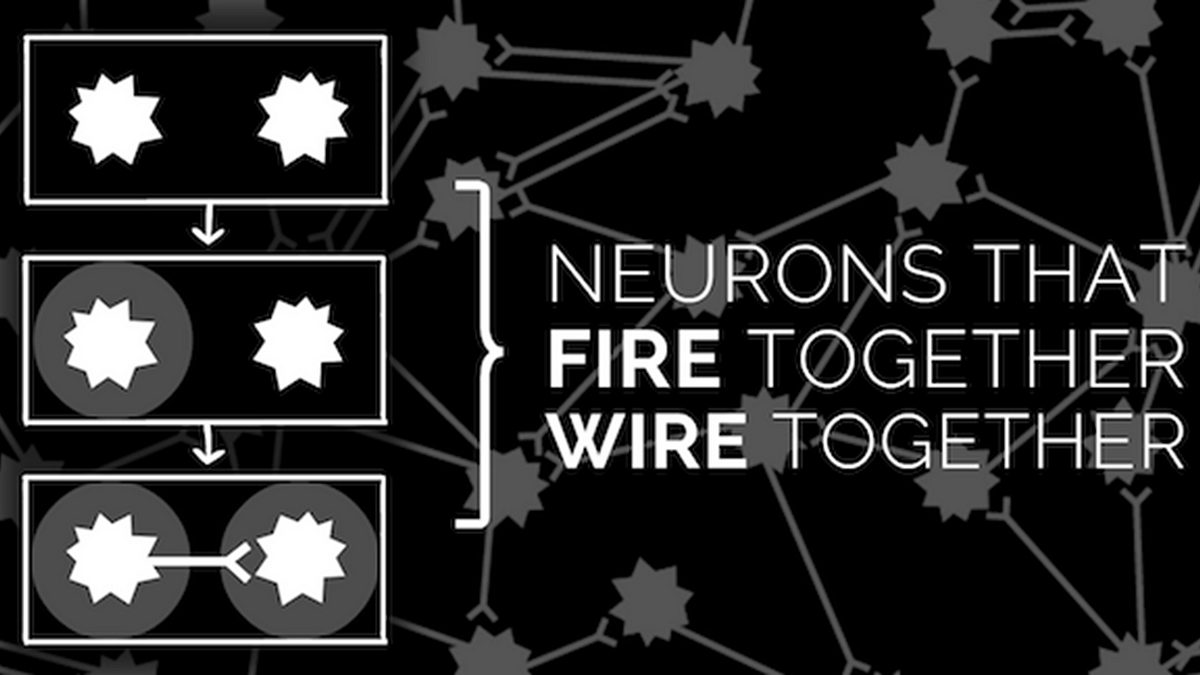
\includegraphics[width=.5\linewidth]{figure/hebbian.png}
        \caption{The principle of Hebbian learning.}
    \end{figure}
    \begin{itemize}
        \item Hebbian update rule: $\mathbf{S}_t = \mathbf{S}_{t-1} + \mathbf{v}_t \mathbf{k}_t^\top$
        \item Delta rule: $\mathbf{S}_t = \mathbf{S}_{t-1} - \beta_t \left(\mathbf{S}_{t-1} \mathbf{k}_t - \mathbf{v}_t\right) \mathbf{k}_t^\top$
        \item ...
    \end{itemize}
    Both Hebbian and delta update rules can be regarded as optimizing online learning objective via {\color{red}test-time SGD}.


\end{frame}
\begin{frame}{Linear Attention: Test-Time Objective}
    \begin{center}
    \begin{tikzpicture}
        \begin{scope}[xshift=3cm]
            \node at (0,3.5) {Maximize alignment};
            \node at (0,3) {= Minimize angle difference + enlarge $|\mathbf{S}\mathbf{k}|$};
            
            \coordinate (O) at (0,0);
            \draw[->,purple,thick] (O) -- (1.75,1.75) coordinate (Mk) node[above] {$\mathbf{S}_{t-1}\mathbf{k}_t$};
            \draw[->,blue,thick] (O) -- (1.5,0.8) coordinate (v) node[right] {$\mathbf{v}_t$};
            
            \draw[->, purple,dashed] (O) -- (3,2.1) node[above] {$\mathbf{S}_{t}\mathbf{k}_t$};
    
            \draw[dashed] (-1,0) -- (2,0);
            \draw[dashed] (0,-1) -- (0,2);
            
            \pic [draw, angle radius=5mm] {angle = v--O--Mk};
        \end{scope}
    \end{tikzpicture}
    \end{center}
\vspace{-2mm}
    \begin{align*}
\hspace*{-1cm}\textbf{Objective: } & \mathcal{L}_t(\mathbf{S}) = -\langle \mathbf{S} \mathbf{k}_t, \mathbf{v}_t \rangle \\[1ex]
\hspace*{-1cm}\textbf{SGD update: } & \mathbf{S}_t = \mathbf{S}_{t-1} - \beta_t \nabla \mathcal{L}_t(\mathbf{S}_{t-1}) = \mathbf{S}_{t-1} + \beta_t \mathbf{v}_t \mathbf{k}_t^\top
    \end{align*}
    \vspace{-6mm}

\end{frame}

\begin{frame}{Linear Attention: Test-Time Objective}
    \begin{center}
        \begin{tikzpicture}
            \begin{scope}[xshift=3cm]
                \node at (0,3.5) {Maximize alignment};
                \node at (0,3) {= Minimize angle difference + enlarge $|\mathbf{S}\mathbf{k}|$};
                
                \coordinate (O) at (0,0);
                \draw[->,purple,thick] (O) -- (1.75,1.75) coordinate (Mk) node[above] {$\mathbf{S}_{t-1}\mathbf{k}_t$};
                \draw[->,blue,thick] (O) -- (1.5,0.8) coordinate (v) node[right] {$\mathbf{v}_t$};
                
                \draw[->, purple,dashed] (O) -- (3,2.1) node[above] {$\mathbf{S}_{t}\mathbf{k}_t$};
        
                \draw[dashed] (-1,0) -- (2,0);
                \draw[dashed] (0,-1) -- (0,2);
                
                \pic [draw, angle radius=5mm] {angle = v--O--Mk};
            \end{scope}
        \end{tikzpicture}
        \end{center}
        \vspace{-4mm}
    \begin{itemize}
        \item Linear attention may favor increasing $|\mathbf{S}\mathbf{k}|$ over angle alignment, leading to numerical instabilities.
        \item Mamba2 uses {\color{red}decay} ($\mathbf{S}_t = {\color{red}\alpha_t} \mathbf{S}_{t-1} + \mathbf{v}_t \mathbf{k}_t^\top$) to control $|\mathbf{S}\mathbf{k}|$, stabilizing the training process.
    \end{itemize}
\end{frame}

\begin{frame}{DeltaNet: Test-Time Objective}
    \begin{center}
        \begin{tikzpicture}[scale=0.9]
            \begin{scope}[xshift=1cm]  
                \node at (0,3.5) {Directly minimize Euclidean distance};
                
                \coordinate (O) at (0,0);
                \draw[dashed] (-2,0) -- (3,0);     
                \draw[dashed] (0,-1) -- (0,3);     
                
                % Original vectors - 调整位置使更分散
                \draw[->,purple,thick] (O) -- (2,2) coordinate (Mk1) node[above] {$\mathbf{S}_{t-1}\mathbf{k}_t$};
                \draw[->,blue,thick] (O) -- (1.5,0.8) coordinate (v) node[right] {$\mathbf{v}_t$};
                
                % Draw the distance line - 需要更新坐标以匹配新的向量位置
                \draw[thick] (2,2) -- (1.5,0.8);
                
                % Dashed vector halfway between Mk1 and v - 调整位置
                \draw[->, purple,dashed] (O) -- (1.75,1.4) node[right] {$\mathbf{S}_{t}\mathbf{k}_t$};
            \end{scope}
        \end{tikzpicture}
     \end{center}
\vspace{-5mm}      
% DeltaNet (\cite{Schlag2021LinearTA, yang2024parallelizing}) optimizes a regression loss via SGD:
    \begin{align*}
        \textbf{Objective: } & \mathcal{L}_t(\mathbf{S}) = \frac{1}{2}\|\mathbf{S} \mathbf{k}_t - \mathbf{v}_t\|^2 \\[1ex]
        \textbf{SGD update: } & \mathbf{S}_t = \mathbf{S}_{t-1} - \beta_t \nabla \mathcal{L}_t(\mathbf{S}_{t-1}) = \mathbf{S}_{t-1} - \beta_t (\mathbf{S}_{t-1} \mathbf{k}_t - \mathbf{v}_t)\mathbf{k}_t^\top 
    \end{align*}
    \vspace{-5mm}

        \begin{itemize}
            \item {\color{red} Better numerical stability}: the norm of $\mathbf{S}_t$ is controlled.
            \item {\color{red} Better in-context associative recall}: directly optimizes key-value association prediction (\cite{Liu2024LonghornSS})
        \end{itemize}




    % Online regression loss is better for predicting $\mathbf{v}_t$ from $\mathbf{k}_t$ and $\mathbf{S}_{t-1}$.
    %     $$\mathcal{L}_t(\mathbf{S}) = \frac{1}{2}\|\mathbf{S} \mathbf{k}_t - \mathbf{v}_t\|^2$$
    %     \vspace{2mm}
    %     Performing a single step of SGD:
    % $$\begin{aligned}
    % \mathbf{S}_t &= \mathbf{S}_{t-1} - \beta_t \nabla \mathcal{L}_t(\mathbf{S}_{t-1}) \\
    % &= \mathbf{S}_{t-1} - \beta_t \left(\mathbf{S}_{t-1} \mathbf{k}_t - \mathbf{v}_t\right) \mathbf{k}_t^\top
    % \end{aligned}$$
    % \begin{itemize}
    %     \item When $\beta_t \in (0, 1)$, the DeltaNet update rule (\cite{Schlag2021LinearTA, yang2024parallelizing}) is recovered.  
    % \end{itemize}
\end{frame}

% \begin{frame}{Comparison between DeltaNet and Linear Attention}
%     \begin{tikzpicture}
%         % Title
%         % Left diagram
%         \begin{scope}[xshift=-4cm]
%             \node at (0,3.5) {Maximize ``alignment''};
%             \node at (0,3) {= Minimize angle + enlarge $|Mk|$};
            
%             % Define coordinates and draw vectors with names
%             \coordinate (O) at (0,0);
%             \draw[->,purple,thick] (O) -- (1.75,1.75) coordinate (Mk) node[above] {$\mathbf{S}_{t-1}\mathbf{k}_t$};
%             \draw[->,green,thick] (O) -- (1.5,0.8) coordinate (v) node[right] {$\mathbf{v}_t$};
            
%             % Add dashed extension to show enlarging norm
%             \draw[->, purple,dashed] (O) -- (3,2.1) node[above] {$\mathbf{S}_{t}\mathbf{k}_t$};
%             % \node[right] at (2.0,2.0) {$\uparrow$};
    
%             % Coordinate axes
%             \draw[dashed] (-1,0) -- (2,0);
%             \draw[dashed] (0,-1) -- (0,2);
            
%             % Draw angle arc
%             \pic [draw, angle radius=5mm] {angle = v--O--Mk};
            
%             % Loss function
%             \node at (0,-1.5) {$\text{loss}_M(k,v) = -\langle \mathbf{S}_{t-1}\mathbf{k}_t, \mathbf{v}_t \rangle$};
%         \end{scope}
        
%         % Right diagram
%         \begin{scope}[xshift=2cm]
%             \node at (0,3.5) {Minimize (Euclidean) distance};
            
%             \coordinate (O) at (0,0);
%             \draw[dashed] (-1,0) -- (2,0);
%             \draw[dashed] (0,-1) -- (0,2);
            
%             % Original vectors
%             \draw[->,purple,thick] (O) -- (1.75,1.75) coordinate (Mk1) node[above] {$\mathbf{S}_{t-1}\mathbf{k}_t$};
%             \draw[->,green,thick] (O) -- (1.5,0.8) coordinate (v) node[right] {$\mathbf{v}_t$};
            
%             % Draw the distance line
%             \draw (1.75,1.75) -- (1.5,0.8);
            
%             % Dashed vector halfway between Mk1 and v
%             \draw[->, purple,dashed] (O) -- (1.6,1.3) node[right] {$\mathbf{S}_{t}\mathbf{k}_t$};
            
%             \node at (0,-1.5) {$\mathcal{L}_{S}(k,v) = \frac{1}{2}\|\mathbf{S}_{t-1}\mathbf{k}_t - \mathbf{v}_t\|^2$};
%         \end{scope}
%     \end{tikzpicture}
%     \begin{itemize}
%         \item Linear attention's objective encourages expanding the norm of $\mathbf{S}_t$, leading to numerical instabilities. 
%         \begin{itemize}
%             \item Weight decay (e.g., in Mamba2) could mitigate this issue.
%         \end{itemize}
%         \item DeltaNet's objective encourages minimizing the distance between $\mathbf{S}_t \mathbf{k}_t$ and $\mathbf{v}_t$, which is more stable.
%     \end{itemize}
% \end{frame}
% \begin{frame}{DeltaNet performs better on in-context associative recall}
%     \begin{block}{Associative recall}
%         \begin{quote}
%             \small ``In psychology, associative memory is {\color{red} \textbf{the ability to learn and remember relationships between unrelated items}}, such as remembering someone's name when seeing their face. This allows us to form connections between distinct pieces of information.''
%         \end{quote}
%     \end{block}
    
%     DeltaNet learns associations through online linear regression: minimizing $\|\mathbf{S}\mathbf{k}_i - \mathbf{v}_i\|^2$ directly optimizes key-value prediction (\cite{Liu2024LonghornSS}).
% \end{frame}

\begin{frame}{In-context associative recall}
    \begin{block}{\scriptsize Multi-Query Associative Recall (MQAR, \cite{zoology})}
        \scriptsize
        A synthetic benchmark for testing in-context associative recall.
        \vspace{1mm}
        \textbf{Example:}
        \begin{itemize}
            \item Given key-value pairs: ``A 4 B 3 C 6 F 1 E 2''
            \item Query: ``A ? C ? F ? E ? B ?''  
            \item Expected output: ``4, 6, 1, 2, 3''
        \end{itemize}
    \end{block}
    \vspace{-1mm}
    
% \definecolor{color1}{RGB}{145,30,180}
% \definecolor{color2}{RGB}{245,130,48}
% \definecolor{color3}{RGB}{230,25,75}
% \definecolor{color4}{RGB}{123,25,75}
% \definecolor{color5}{RGB}{44,160,44}

\definecolor{color1}{RGB}{116, 184, 22}
\definecolor{color2}{RGB}{77, 171, 247}
\definecolor{color3}{RGB}{99, 230, 190}
\definecolor{color4}{RGB}{132, 94, 247}
\definecolor{color5}{RGB}{250, 176, 5}

\begin{figure}
    \centering
    \resizebox{.5\columnwidth}{!}{  
        \begin{tikzpicture}
        \begin{axis}[
            name=plot2,
            sharp plot,
            title style={align=right},
            title={Sequence Length: 512, Key-Value Pairs: 64},
            xmode=normal,
            xlabel=Model dimension,
            width=6cm, height=5cm,
            ymin=0, ymax=100,
            symbolic x coords={64,128,256,512},
            ytick={0,25,50,75,100},
            yticklabels={0,25,50,75,100},
            xlabel near ticks,
            ylabel near ticks,
            ylabel=Accuracy (\%),
            ymajorgrids=true,
            xmajorgrids=true,
            grid style=dashed,
            legend style={at={(1.6,0.5)},anchor=east, legend cell align=left, font=\small}, 
        ]

        \addplot[very thick, mark=square*, mark options={scale=1}, color=red] plot coordinates {
            (64,100)
            (128,100)
            (256,100)
            (512,100)
        };
        \addlegendentry{DeltaNet} 

        \addplot[very thick,mark=+,mark options={scale=1}, color=color1] plot coordinates { 
            (64,81)
            (128,100)
            (256,100)
            (512,100)
        };
        \addlegendentry{Mamba} 
        
        \addplot[very thick, mark=square*, mark options={scale=1}, color=color2] plot coordinates {
            (64,22)
            (128,95)
            (256,100)
            (512,100)
        };
        \addlegendentry{GLA} 
        
        \addplot[very thick, mark=star, mark options={scale=1}, color=color3] plot coordinates {
            (64,5)
            (128,87)
            (256,96)
            (512,97)
        };
        \addlegendentry{RetNet}  

        \addplot[very thick, mark=+, mark options={scale=1}, color=color4] plot coordinates {
            (64,0)
            (128,0)
            (256,20)
            (512,35)
        };
        \addlegendentry{RWKV4}  

        \addplot[very thick, mark=o, mark options={scale=1}, color=color5] plot coordinates {
            (64,0)
            (128,0)
            (256,12)
            (512,20)
        };
        \addlegendentry{Hyena} 

        \end{axis}
        \end{tikzpicture}
    }
    \vspace{-3.5mm}
    \caption{Accuracy (\%) on MQAR. DeltaNet achieves the perfect recall.} 
    \label{fig:mqar} 
\end{figure}
\end{frame}
% \begin{frame}{DeltaNet performs better on in-context associative recall: MAD results}
%     MAD (\cite{poli_mechanistic_2024}) serves as a more comprehensive benchmark suite than MQAR for evaluating in-context associative recall and learning.
%     \begin{table}
% \resizebox{\linewidth}{!}{
% \begin{tabular}{l|*{6}{c}|c}
% \toprule
% \textbf{Model} & \textbf{Compress} & \cellcolor{red!15}\textbf{Fuzzy} & \cellcolor{red!15}\textbf{In-Context} & \textbf{Memorize} & \cellcolor{red!15}\textbf{Noisy} & \cellcolor{red!15}\textbf{Selective} & \textbf{Average} \\
% & & \cellcolor{red!15}\textbf{Recall} & \cellcolor{red!15}\textbf{Recall} & & \cellcolor{red!15}\textbf{Recall} & \cellcolor{red!15}\textbf{Copy} & \\
% \midrule
% Transformer & 51.6 & \cellcolor{red!15}29.8 & \cellcolor{red!15}94.1 & 85.2 & \cellcolor{red!15}86.8 & \cellcolor{red!15}99.6 & 74.5 \\
% Hyena & 45.2 & \cellcolor{red!15}7.9 & \cellcolor{red!15}81.7 & 89.5 & \cellcolor{red!15}78.8 & \cellcolor{red!15}93.1 & 66.0 \\
% Multihead Hyena \hspace{4mm} & 44.8 & \cellcolor{red!15}14.4 & \cellcolor{red!15}99.0 & 89.4 & \cellcolor{red!15}98.6 & \cellcolor{red!15}93.0 & 73.2 \\
% Mamba & 52.7 & \cellcolor{red!15}6.7 & \cellcolor{red!15}90.4 & 89.5 & \cellcolor{red!15}90.1 & \cellcolor{red!15}86.3 & 69.3 \\
% GLA & 38.8 & \cellcolor{red!15}6.9 & \cellcolor{red!15}80.8 & 63.3 & \cellcolor{red!15}81.6 & \cellcolor{red!15}88.6 & 60.0 \\
% DeltaNet & 42.2 & \cellcolor{red!15}\textbf{35.7} & \cellcolor{red!15}\textbf{100} & 52.8 & \cellcolor{red!15}\textbf{100} & \cellcolor{red!15}\textbf{100} & 71.8 \\
% \bottomrule
% \end{tabular}
% }
% \caption{MAD benchmark results. DeltaNet achieves the best performance in in-context associative recall and copy tasks, however, it somehow underperforms in memorization and compression tasks.}
% \label{tab:mad_results}
% \end{table}
% \end{frame}


\begin{frame}{Transformers and SSMs in TC$^0$}
    \begin{figure}
        \centering
        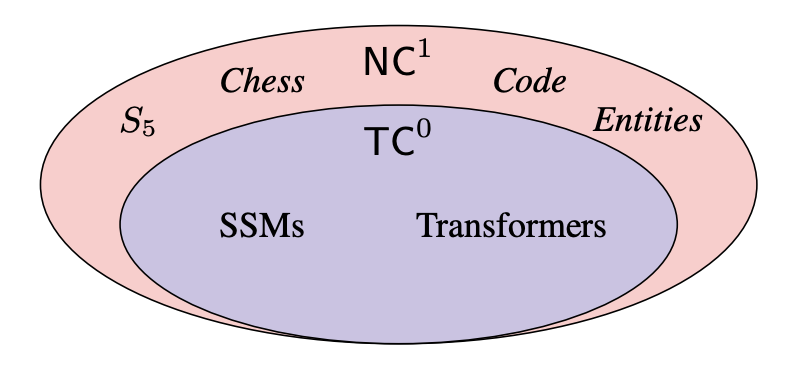
\includegraphics[width=.45\linewidth]{figure/tc0.png}
    \end{figure}
    \vspace{-2mm}
\begin{itemize}
    \item Transformers are in TC$^0$.
    \item Linear RNNs with {\color{red}diagonal transition matrices} (e.g., $\mathbf{S}_t = \mathbf{S}_{t-1} \operatorname{diag}(\boldsymbol{\alpha}_t) + \mathbf{v}_t \mathbf{k}_t^\top$ in GLA) fall under TC$^0$.
    \item {\color{red} Nonlinear RNN} or linear RNN with {\color{red} data-dependent nondiagonal transition matrices} could achieve expressiveness beyond TC$^0$ (\cite{Merrill2024TheIO}).
\end{itemize}
\end{frame}

\begin{frame}{DeltaNet's expressiveness}
    \begin{align*}
    \mathbf{S}_t &= \mathbf{S}_{t-1} - \beta_t \left(\mathbf{S}_{t-1} \mathbf{k}_t - \mathbf{v}_t\right) \mathbf{k}_t^\top \\
    &= \mathbf{S}_{t-1} {\color{blue}\left(\mathbf{I} - \beta_t \mathbf{k}_t \mathbf{k}_t^\top\right)} + \beta_t \mathbf{v}_t \mathbf{k}_t^\top
    \end{align*}

    DeltaNet uses {\color{blue} Generalized Householder} (GH) transition matrices, which are both {\color{red}data-dependent} and {\color{red}nondiagonal}, making it possible to achieve expressiveness beyond $TC^0$.
    % {\color{red}Both conditions} are necessary to achieve expressiveness beyond $TC^0$ (\cite{Merrill2024TheIO}).
\end{frame}



 \begin{frame}{DeltaNet's expressiveness}
    % First show the state update equation
    \begin{align*}
        \mathbf{S}_t &= \mathbf{S}_{t-1} \underbrace{(\mathbf{I} - \beta_t \mathbf{k}_t \mathbf{k}_t^\top)}_{\text{GH transition}} + \beta_t \mathbf{v}_t \mathbf{k}_t^\top 
        = \sum_{i=1}^{t} \left(\beta_i \mathbf{v}_i \mathbf{k}_i^t {\color{blue}\underbrace{\prod_{j=i+1}^{t} (\mathbf{I} - \beta_j \mathbf{k}_j \mathbf{k}_j^\top)}_{\text{cumulative GH products}}}\right)
    \end{align*}

    \vspace{-8mm}
    
    \textbf{Key Properties:}
    \begin{itemize}
        
        \item \textbf{Expressiveness}: When allowing negative eigenvalues in GH matrices (\cite{Grazzi2024UnlockingSI}), {\color{blue}the cumulative products of GH matrices} can represent \textit{any} matrix with Euclidean norm < 1.
        
        \item \textbf{Complexity Class}: 
            {\color{blue}Cumulative products of general matrices} cannot be computed in TC$^0$ (\cite{Mereghetti2000ThresholdCF}).

        \item \textbf{Conclusion}: {\color{red}DeltaNet with negative eigenvalues has expressiveness beyond TC$^0$}, strictly exceeding SSMs and Transformers.
    \end{itemize}
\end{frame}
    

\begin{frame}{State tracking performance}
    \begin{figure}
        \centering
        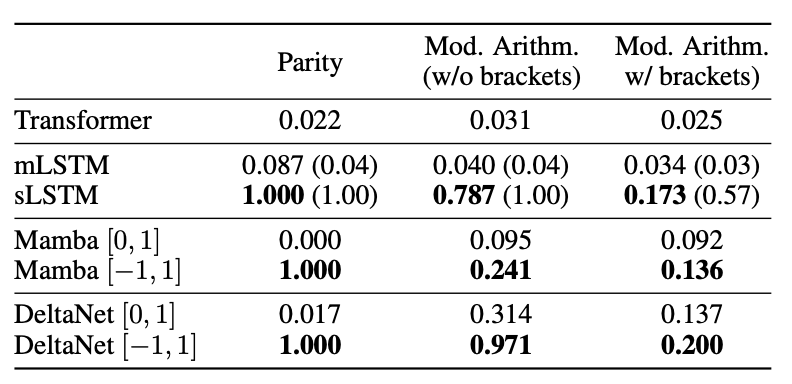
\includegraphics[width=.75\linewidth]{figure/state_tracking.png}
        \caption{State tracking performance comparison (source: \cite{Grazzi2024UnlockingSI}). $[0,1]$ and $[-1,1]$ denotes the ranges of eigenvalues for each model's transition matrix.}
    \end{figure}
    \vspace{-5mm}
   \begin{itemize}
    \item {\color{red}Allowing negative eigenvalues} could boost state tracking performance for both Mamba and DeltaNet.
    \item DeltaNet achieves superior performance due to its {\color{red}richer expressiveness}.
   \end{itemize}
\end{frame}

\begin{frame}{DeltaNet: Chunkwise Parallel Training}
    \begin{align*}
        \mathbf{S}_t &= \mathbf{S}_{t-1} \left(\mathbf{I} - \beta_t \mathbf{k}_t \mathbf{k}_t^\top\right) + \beta_t \mathbf{v}_t \mathbf{k}_t^\top \\
        &= \mathbf{S}_{t-1} + {\color{red}\underbrace{\beta_t(\mathbf{v}_t - \mathbf{S}_{t-1} \mathbf{k}_t)}_{\text{defined as } \mathbf{u}_t}} \mathbf{k}_t^\top \\
        &= \mathbf{S}_{t-1} + {\color{red}\mathbf{u}_t} \mathbf{k}_t^\top \\
        &= \sum_{i=1}^{t} {\color{red}\mathbf{u}_i} \mathbf{k}_i^\top
    \end{align*}    Once ``pseudo-values'' ${\color{red}\mathbf{u}_t}$ are computed, DeltaNet can be trained using the same kernel as linear attention.
\end{frame}


\begin{frame}{DeltaNet: Chunkwise Parallel Training}
    \begin{align*}
        \mathbf{S}_t &= \mathbf{S}_{t-1} \left(\mathbf{I} - \beta_t \mathbf{k}_t \mathbf{k}_t^\top\right) + \beta_t \mathbf{v}_t \mathbf{k}_t^\top \\
        &= \sum_{i=1}^{t} \left(\beta_i \mathbf{v}_i \mathbf{k}_i^\top {\color{blue}\underbrace{\prod_{j=i+1}^{t} (\mathbf{I} - \beta_j \mathbf{k}_j \mathbf{k}_j^\top)}_{\mathbf{P}_j^t}}\right) 
    \end{align*}
    Using the WY representation (\cite{bischof_wy_1985}):
    \[
    \color{blue}\mathbf{P}_{1}^t = \mathbf{I} - \sum_{i=1}^{t}\mathbf{w}_{i}\mathbf{k}_{i}^{\top}.
    \]
    \color{black}
    {\color{red}\textbf{Key Insight}}: The cumulative product $\prod$ becomes a cumulative sum $\sum$, enabling efficient matrix-multiply-based training.
    \end{frame}

\begin{frame}{}
\vspace{-2mm}
    \scalebox{1.0}{
\begin{tikzpicture}
    \foreach \x in {0,5,10,15} {
        \draw[dashed] (\x,-2) -- (\x,2);
    }

        \begin{scope}[shift={(-1.5,0)}]
            \node[draw=black, minimum size=1cm] (grid-0-3) at (0.5,0.5) {};
            \foreach \x in {0,0.33,0.66} {
                \foreach \y in {0,0.33,0.66} {
                    \draw[black] (\x+0.17,\y+0.17) circle (0.12);
                }
            }
        \end{scope}

    \foreach \section [count=\i] in {0.5,5.5} {
        \foreach \offset [count=\j] in {0,1.5} {
            \begin{scope}[shift={(\section+\offset,0)}]
                \node[draw=gray!30, minimum size=1cm] (grid-\i-\j) at (0.5,0.5) {};
                \foreach \x in {0,0.33,0.66} {
                    \foreach \y in {0,0.33,0.66} {
                        \draw[gray!30] (\x+0.17,\y+0.17) circle (0.12);
                    }
                }
            \end{scope}
        }
        
        \begin{scope}[shift={(\section+3,0)}]
            \node[draw=black, minimum size=1cm] (grid-\i-3) at (0.5,0.5) {};
            \foreach \x in {0,0.33,0.66} {
                \foreach \y in {0,0.33,0.66} {
                    \draw[black] (\x+0.17,\y+0.17) circle (0.12);
                }
            }
        \end{scope}
    }
    
    \foreach \section [count=\i] in {0.5,5.5} {
        \begin{scope}[shift={(\section,-1.5)}]
            \foreach \offset [count=\j] in {0,1.5,3} {
                \node[fill=blue!20,draw=black, minimum width=1cm, minimum height=0.4cm] (rect-\i-\j) at (\offset+0.5,0.2) {};
                \foreach \x in {0.2, 0.5, 0.8} {
                    \draw[black] (\offset+\x,0.2) circle (0.1);
                }
                \draw[->,red!30,very thick] (rect-\i-\j.north) to[out=90,in=-90, looseness=0.7] 
                    ([xshift=\j*0cm]grid-\i-3.south);
            }

        \end{scope}
    }
    
\draw[->,yellowgreen,very thick] (grid-0-3.east)  to[bend left=60] (grid-1-3.west);
\draw[->,yellowgreen,very thick] (grid-1-3.east)  to[bend left=60] node[above,xshift=-1.5cm, yshift=0cm,align=center]{
  \textcolor{black}{{\large{\textbf{\color{red}Sequential}} Chunk-Level State Passing:}} 
%   $\color{black}\boldsymbol{S}_{[t+1]}=\boldsymbol{S}_{[t]}
    % {\color{blue!50}\colorbox{yellowgreen!30}{$\mathrlap{({\boldsymbol{I}}-\boldsymbol{W}_{[t]}^\top \boldsymbol{K}_{[t]})}$}} + 
    % {\color{blue!50}\colorbox{red!30}{$\mathrlap{\boldsymbol{U}_{[t]}^\top \boldsymbol{K}_{[t]}}$}}$
} (grid-2-3.west);


\end{tikzpicture}
}

    \vspace{-10mm}
    \begin{align*}
        \boldsymbol{S}_{[t+1]} &= \boldsymbol{S}_{[t]}
        {\color{blue!50}\colorbox{yellowgreen!30}{$\mathbf{({\boldsymbol{I}}-\boldsymbol{W}_{[t]}^\top \boldsymbol{K}_{[t]})}$}} + 
        {\color{blue!50}\colorbox{red!30}{$\mathbf{\boldsymbol{U}_{[t]}^\top \boldsymbol{K}_{[t]}}$}}
    \end{align*}
 Using hardware-friendly UT transform (\cite{Joffrain2006AccumulatingHT}):
    \begin{align*}
        \mathbf{T}_{[t]} &= \left(\mathbf{I} + \operatorname{tril}(\operatorname{diag}(\beta_{[t]})\mathbf{K}_{[t]} \mathbf{K}_{[t]}^\intercal,-1)\right)^{-1}\operatorname{diag}\left(\beta_{[t]}\right) &&\in \mathbb{R}^{C \times C} \\  \mathbf{W}_{[t]} &= \mathbf{T}_{[t]} \mathbf{K}_{[t]}, \quad 
        \mathbf{U}_{[t]}=\mathbf{T}_{[t]}\mathbf{V}_{[t]} && \in \mathbb{R}^{C \times d}
    \end{align*}

    \begin{tcolorbox}[colback=yellowgreen!30,colframe=black,boxrule=0.5pt]
        \footnotesize See \url{https://sustcsonglin.github.io/blog/2024/deltanet-2/} for details.
    \end{tcolorbox}
\end{frame}

\begin{frame}{}
    
\begin{tikzpicture}[
    box/.style={
        rectangle,
        minimum size=0.5cm,
        draw=black!20
    }
]
    \foreach \x in {0,5,10,15} {
        \draw[dashed] (\x,-2) -- (\x,2);
    }
            \begin{scope}[shift={(-1.5,0)}]
            \node[draw=black, minimum size=1cm] (grid-0-3) at (0.5,0.5) {};
            \foreach \x in {0,0.33,0.66} {
                \foreach \y in {0,0.33,0.66} {
                    \draw[black] (\x+0.17,\y+0.17) circle (0.12);
                }
            }
        \end{scope}


    \foreach \section [count=\i] in {0.5,5.5} {

        % \foreach \offset [count=\j] in {0,1.5} {

     \begin{scope}[shift={(\section+1.5,0.1)}]

        \node[box, fill=red!100, minimum size=0.33cm] at (0.17,0.83) {};
        \node[box, minimum size=0.33cm] at (0.5,0.83) {};
        \node[box, minimum size=0.33cm] at (0.83,0.83) {};
        
        \node[box, fill=red!15, minimum size=0.33cm] at (0.17,0.5) {};
        \node[box, fill=red!75, minimum size=0.33cm] at (0.5,0.5) {};
        \node[box, minimum size=0.33cm] at (0.83,0.5) {};
        

        \node[box, fill=red!25, minimum size=0.33cm] at (0.17,0.17) {};
        \node[box, fill=red!45, minimum size=0.33cm] (attn-\i)at (0.5,0.17) {};
        \node[box, fill=red!65, minimum size=0.33cm] at (0.83,0.17) {};
    \end{scope}

        \begin{scope}[shift={(\section+3,0)}]
            \node[draw=black, minimum size=1cm] (grid-\i-3) at (0.5,0.5) {};
            \foreach \x in {0,0.33,0.66} {
                \foreach \y in {0,0.33,0.66} {
                    \draw[black] (\x+0.17,\y+0.17) circle (0.12);
                }
            }
        \end{scope}
    }
    

    \foreach \section [count=\i] in {0.5,5.5} {
        \begin{scope}[shift={(\section,-1.5)}]

            \foreach \offset [count=\j] in {0,1.5,3} {
                \node[draw=black, fill=blue!20, minimum width=1cm, minimum height=0.4cm] (rect-\i-\j) at (\offset+0.5,0.2) {};

                \foreach \x in {0.2, 0.5, 0.8} {
                    \draw[black] (\offset+\x,0.2) circle (0.1);
                }
                \node[draw=black, minimum width=1cm, minimum height=0.4cm,fill=orange!30] (upper-rect-\i-\j) at (\offset+0.5,0.2+3.5) {};
                \foreach \x in {0.2, 0.5, 0.8} {
                    \draw[black] (\offset+\x,0.2+3.5) circle (0.1);
                }
                
            
    \pgfmathsetmacro{\prevsection}{\i-1}
\draw[->, yellowgreen, thick] 
    (grid-\the\numexpr\i-1\relax-3.east) 
    to[bend left=20] 
    (upper-rect-\i-\j.west);

\draw[->, yellowgreen, thick] 
    (rect-\i-\j.north) 
    to[bend left=30] 
    (upper-rect-\i-\j.west);

\draw[->,red!50,very thick] (rect-\i-\j.north) to[out=90,in=-90,looseness=1.2] (attn-\i.south);

\draw[->,red!50,very thick] ([yshift=0.6cm]attn-\i.north) to[out=90,in=-90,looseness=1.2] (upper-rect-\i-\j.south);

}

\ifnum\i>1
\fi

        \end{scope}
    }
    
\node[above=0.25cm,xshift=-3cm,align=center] at (upper-rect-2-2.north) {
  \textcolor{black}{\large{\textbf{\color{red}Parallel} Output Computation:}} \\
%   ${\color{orange}\mathbf{O}_{[i]}}=\colorbox{yellowgreen!30}{${\color{blue!50}\mathbf{Q}_{[i]}}\mathbf{S}_{[i]}^\top$}+\colorbox{red!30}{\color{blue!50}$\left({\mathbf{Q}_{[i]}\mathbf{K}_{[i]}^\top \odot \mathbf{M}}\right)\mathbf{V}_{[i]}$}$
};

\end{tikzpicture}

      \begin{align*}
        {\color{orange}\mathbf{O}_{[t]}} &= \colorbox{yellowgreen!30}{${\color{blue!50}\mathbf{Q}_{[t]}}\mathbf{S}_{[t]}^\top$} + \colorbox{red!30}{$\left({\color{blue!50}\mathbf{Q}_{[t]}\mathbf{K}_{[t]}^\top \odot \mathbf{M}}\right)\left({\color{blue!50}\mathbf{U}_{[t]}}-{\color{blue!50}\mathbf{W_{[t]}}}\mathbf{S_{[t]}^\top} \right)$}
      \end{align*}
      
      Compared to vanilla linear attention, the ``pseudo-values'' need to be adjusted by the historical context: $\mathbf{W}_{[t]}\mathbf{S}_{[t]}^\top$.
\end{frame}



\begin{frame}{Gated DeltaNet}
    Enhancing DeltaNet with a {\color{red}{Mamba2-like gating mechanism}} could boost performance on {\color{red}real-world tasks}.
        \begin{align*}
            \mathbf{S}_t = \mathbf{S}_{t-1} \left({\color{red}\alpha_t}(\mathbf{I} - \beta_t \mathbf{k}_t \mathbf{k}_t^\top)\right) + \beta_t \mathbf{v}_t \mathbf{k}_t^\top
        \end{align*}
    \begin{table}[h!]
        \centering
        \resizebox{0.9\linewidth}{!}{%
            \begin{tabular}{lcccc}
                \toprule
                \textbf{Model} & \textbf{ppl} $\downarrow$ & \textbf{LM-eval} $\uparrow$ & \textbf{Recall} $\uparrow$ & \textbf{Long} $\uparrow$ \\
                \midrule
                Mamba1         & 17.92 & 53.12 & 21.0 & 14.6 \\
                Mamba2         & 16.56 & 54.89 & 29.8 & 13.5 \\
                DeltaNet       & 17.72 & 52.14 & 26.2 & 13.6 \\
                Gated DeltaNet & \textbf{16.42} & \textbf{55.32} & \textbf{30.6} & \textbf{16.6} \\
                \bottomrule
            \end{tabular}
        }
        \caption{Performance comparison of different 1.3B models trained on 100B tokens. Source: \cite{yang2024gateddeltanetworksimproving}.}
        \label{tab:model_comparison}
    \end{table}
\end{frame}
\begin{frame}
    \begin{figure}
        \centering
        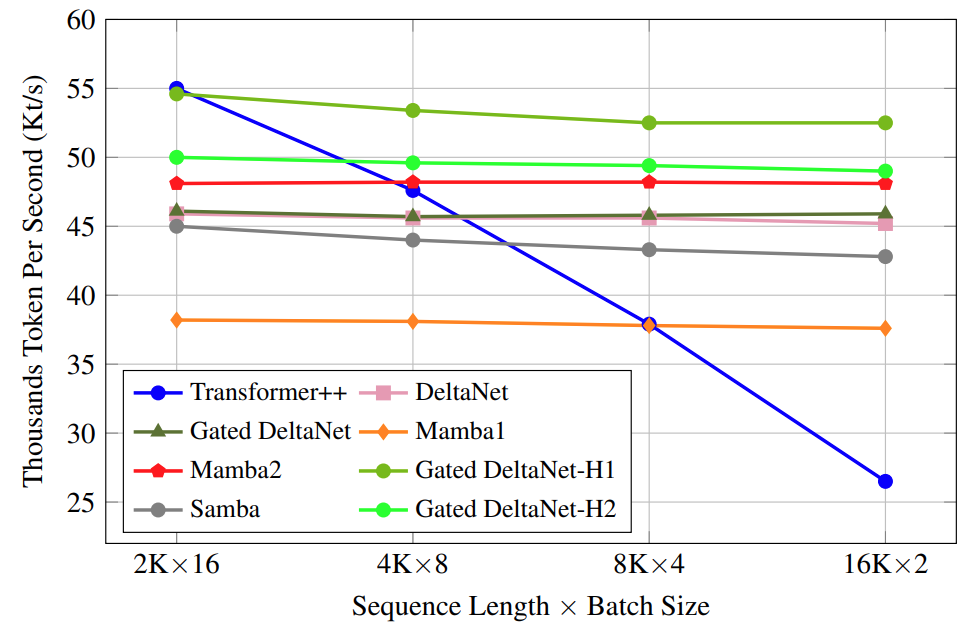
\includegraphics[width=0.65\linewidth]{figure/gdn-speed.png}
        \caption{End-to-end training throughput comparison for different 1.3B models on a single H100. Source: \cite{yang2024gateddeltanetworksimproving}.}
    \end{figure}
    Combining DeltaNet and Mamba2's chunkwise algorithms for hardware-efficient training:
    \begin{itemize}
    \item Pure Gated DeltaNet is slightly slower than Mamba2.  
    \item Hybridizing sliding window attention with Gated DeltaNet (i.e., Gated DeltaNet-H1) improves throughput.
\end{itemize}
\end{frame}

\begin{frame}
    DeltaNet's chunkwise algorithm can be extended to {\color{red}diagonal}-plus-{\color{blue}low-rank} transition matrices:
    \begin{align*}
        \mathbf{S}_t = \mathbf{S}_{t-1} ({\color{red}\mathbf{D}_t} + {\color{blue}\boldsymbol{\alpha}_t \boldsymbol{\beta}_t^\top}) + \mathbf{v}_t \mathbf{k}_t^\top, \quad {\color{red}\mathbf{D}_t \in \mathbb{R}^{d \times d}}, \quad {\color{blue}\boldsymbol{\alpha}_t, \boldsymbol{\beta}_t \in \mathbb{R}^{d}}
    \end{align*}
    \vspace{-5mm}
    \begin{itemize}
        \item \textbf{RWKV-7} employs this linear recurrence, showing effectiveness. 
        \item A fast implementation is available in the flash-linear-attention library (\url{https://github.com/fla-org/flash-linear-attention/blob/main/fla/ops/rwkv7/chunk.py}).
    \end{itemize}
    
    \begin{center}
        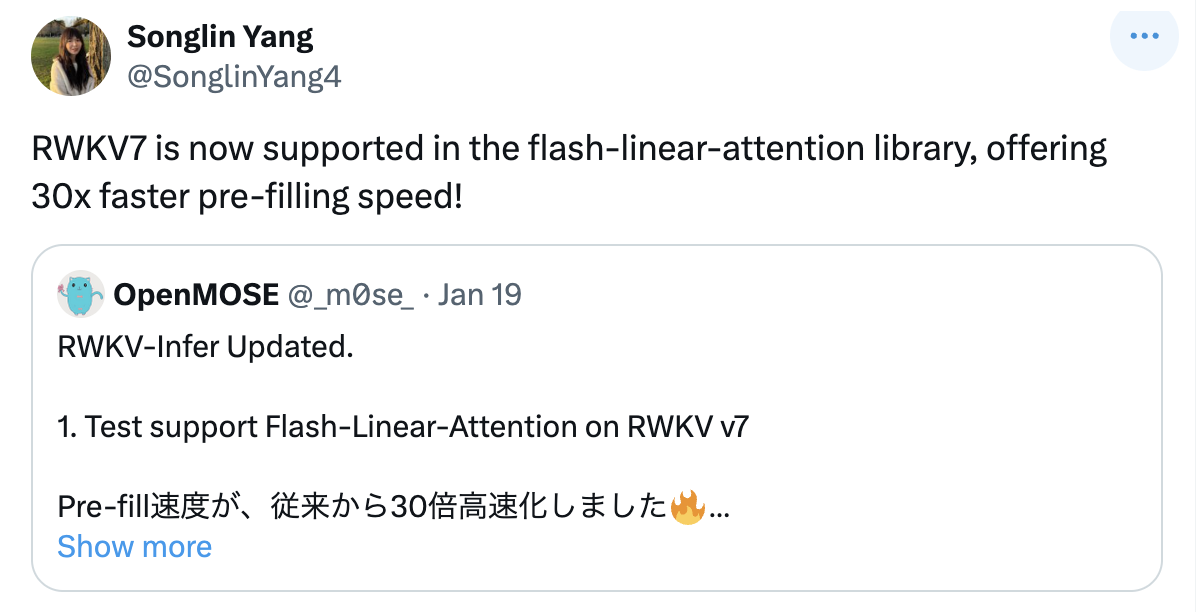
\includegraphics[width=0.75\linewidth]{figure/rwkv7.png}
    \end{center}
\end{frame}

\begin{frame}{DeltaProduct}
    Generalizing the DeltaNet by performing {\color{red}multiple gradient descent steps} (i.e., $n_h$) {\color{blue}per token}:
    \[
    \begin{aligned}
        \mathbf{S}_{{\color{blue}t},{\color{red}j}} &= \mathbf{S}_{{\color{blue}t},{\color{red}j-1}} - \beta_{{\color{blue}t},{\color{red}j}}\nabla\mathcal{L}_{{\color{blue}t},{\color{red}j}}(\mathbf{S}_{{\color{blue}t},{\color{red}j-1}}) \\
        &= \left(\mathbf{I} - \beta_{{\color{blue}t},{\color{red}j}}\mathbf{k}_{{\color{blue}t},{\color{red}j}}\mathbf{k}_{{\color{blue}t},{\color{red}j}}^\top\right)\mathbf{S}_{{\color{blue}t},{\color{red}j-1}} + \beta_{{\color{blue}t},{\color{red}j}}\mathbf{v}_{{\color{blue}t},{\color{red}j}}\mathbf{k}_{{\color{blue}t},{\color{red}j}}^\top
    \end{aligned}
    \]
    where $\mathbf{S}_{{\color{blue}t},{\color{red}0}} = \mathbf{S}_{{\color{blue}t-1}}$ and $\mathbf{S}_{{\color{blue}t},{\color{red}n_h}} = \mathbf{S}_{{\color{blue}t}}$. This results in a \textbf{high-rank} recurrent updates
    \[
    \begin{aligned}
        \mathbf{S}_{\color{blue}t} &= \mathbf{S}_{\color{blue}t-1} \mathbf{A}_{\color{blue}t} + \mathbf{B}_{\color{blue}t} \\
        \mathbf{A}_{\color{blue}t} &= {\color{red}\prod_{j=1}^{n_h}} \left(\mathbf{I} - \beta_{{\color{blue}t}, {\color{red} j}} \mathbf{k}_{{\color{blue}t}, {\color{red} j}} \mathbf{k}_{{\color{blue}t}, {\color{red} j}}^\top\right) \\
        \mathbf{B}_{\color{blue}t} &= {\color{red}\sum_{j=1}^{n_h}} \beta_{{\color{blue}t}, {\color{red} j}} \mathbf{v}_{{\color{blue}t}, {\color{red} j}} \mathbf{k}_{{\color{blue}t}, {\color{red} j}}^\top {\color{red}\prod_{l=1}^{j-1}} \left(\mathbf{I} - \beta_{{\color{blue}t}, {\color{red} l}} \mathbf{k}_{{\color{blue}t}, {\color{red} l}} \mathbf{k}_{{\color{blue}t}, {\color{red} l}}^\top\right)
    \end{aligned}
    \]
    where both the transition matrix $\mathbf{A}_{\color{blue}t}$ and the input $\mathbf{B}_{\color{blue}t}$ are rank-$n_h$ matrices.
\end{frame}

\begin{frame}{DeltaProduct}
    \begin{figure}
        \centering
        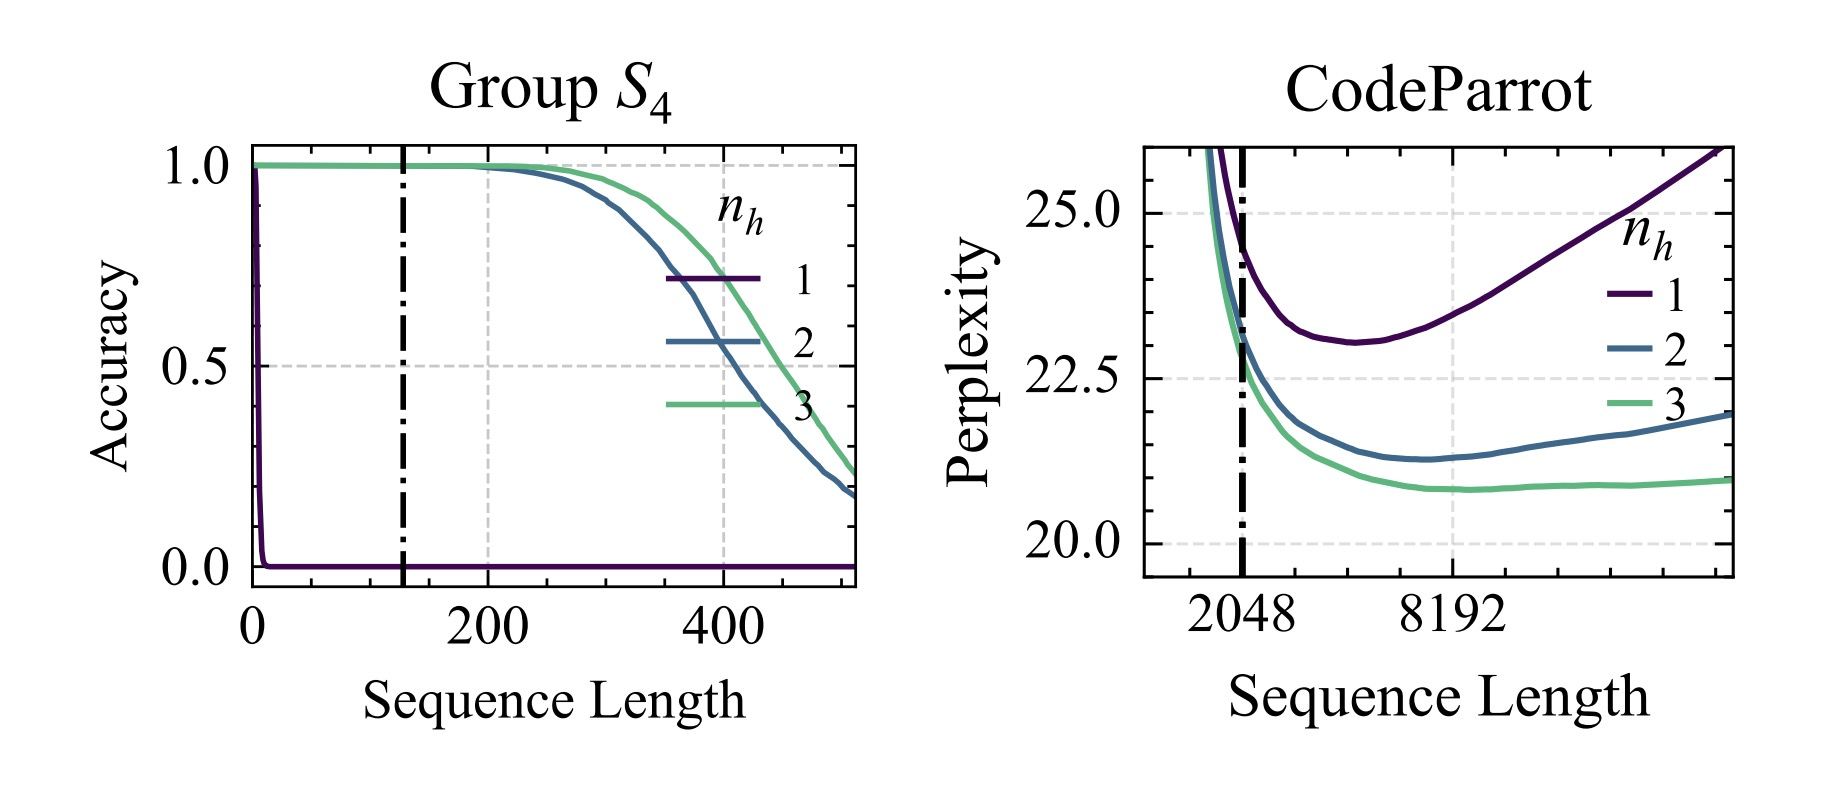
\includegraphics[width=0.9\linewidth]{figure/deltaproduct.jpg}
        \vspace{-4mm}
        \caption{This figure is copied from \cite{siems2025deltaproductincreasingexpressivitydeltanet}.  (\textit{Left}) DeltaProduct$_{n_h}$ learns higher-order permutation groups like $S_4$ in one layer, while DeltaNet ($n_h = 1$) is limited to $S_2$. (\textit{Right}) Length extrapolation of DeltaProduct improves significantly with higher $n_h$.}
    \end{figure}
    
\end{frame}

\begin{frame}{Summary}
    \begin{itemize}
        \item Linear attention and DeltaNet are {\color{red}fast weight programmers} with different {\color{red}test-time SGD} weight updates.
        \item DeltaNet has {\color{red}strictly more expressive power} than Mamba/GLA while {\color{red}maintaining efficient parallelization}
        \item DeltaNet's chunkwise algorithm could be generalized to {\color{red} diagonal-plus-low-rank transition matrices}
        \item {\color{red}Gating} and {\color{red}high-rank updates} further enhance DeltaNet's performance
    \end{itemize}
\end{frame}



\begin{frame}{}
    \centering
    \LARGE
     Beyond linear regression objective
\end{frame}


\begin{frame}{Beyond linear regression objective}
      DeltaNet optimizes the online linear regression loss:
    \begin{align*}
      \mathcal{L}_t(\mathbf{S}) = \frac{1}{2}\|\mathbf{S} \mathbf{k}_t - \mathbf{v}_t\|^2
    \end{align*}
    \begin{itemize}
        \item This optimization objective assumes linear relationships in historical data dependencies
        \item However, generative AI tasks involve complex, nonlinear dependencies
        \item A linear regression loss may be insufficient to capture these rich patterns.
    \end{itemize}
  \end{frame}
  \begin{frame}{Going beyond online linear regression objective}
    TTT (\cite{sun2024learning}) extends this to a nonlinear regression loss:
    \begin{align*}
      \mathcal{L}_t(\mathbf{S}) = \frac{1}{2}\|f_{\mathbf{S}}(\mathbf{k}_t) - \mathbf{v}_t\|^2
    \end{align*}
    where $f_{\mathbf{S}}$ is a nonlinear transformation parameterized by $\mathbf{S}$.

    Examples:
    \begin{itemize}
        \item TTT-linear: 
            \begin{align*}
                f_{\mathbf{S}}(x) = \operatorname{LN}(\mathbf{S}x) + x,
            \end{align*}
        \item TTT-MLP:
            \begin{align*}
                f_{\mathbf{S}}(x) = \operatorname{LN}(\operatorname{MLP}_{\mathbf{S}}(x)) + x
            \end{align*}
    \end{itemize}

    where $\operatorname{LN}$ denotes layer normalization.

    % \begin{itemize}
    %     \item<1-1> \textbf{TTT-linear}: 
    %         \begin{align*}
    %             f_{\mathbf{S}}(x) = \operatorname{LN}(\mathbf{S}x) + x,
    %         \end{align*}
    %         where \(\operatorname{LN}\) denotes layer normalization.
    %         \begin{itemize}
    %             \item \textcolor{red}{\textbf{TTT-linear is a nonlinear RNN}} due to the presence of layer normalization.
    %         \end{itemize}
    
    %     \item<2-2> \textbf{TTT-MLP}:
    %         \begin{align*}
    %             f_{\mathbf{S}}(x) = \operatorname{LN}(\mathbf{S}_2^\top \sigma(\mathbf{S}_1x)) + x,
    %         \end{align*}
    %         where:
    %         \begin{itemize}
    %             \item \( \mathbf{S} = [\mathbf{S}_1 ; \mathbf{S}_2] \) and \( \mathbf{S}_1, \mathbf{S}_2 \in \mathbb{R}^{d \times 4d} \) are analogous to standard MLP layers with an intermediate hidden dimension expansion factor of 4.
    %             \item \( \sigma \) is a nonlinear activation function, and in TTT-MLP, \( \sigma \) is the GeLU activation.
    %         \end{itemize}
    % \end{itemize}
    
  \end{frame}
  \begin{frame}{Beyond Linear Regression Objective}

    The nonlinear loss induces a nonlinear recurrence, posing challenges for parallelization. \\
    \vspace{0.5em}
    \textcolor{red}{\textbf{Solution}}: Mini-batch Gradient Descent
    \begin{itemize}
        \item Minibatch size aligns with chunk size.
        \item Each token within a chunk is treated as an independent training example for parallel processing.
        \item Sequential dependencies are preserved via a lightweight linear recurrence within chunks.
    \end{itemize}
    \vspace{0.5em}
     This approach essentially combines {\color{red}{intra-chunk linear recurrence}} with {\color{red}{inter-chunk nonlinear recurrence}}.
\end{frame}

  \begin{frame}{Beyond linear regression objective}
    TTT (\cite{sun2024learning}) extends this to a nonlinear regression loss:
    \begin{align*}
      \mathcal{L}_t(\mathbf{S}) = \frac{1}{2}\|f_{\mathbf{S}}(\mathbf{k}_t) - \mathbf{v}_t\|^2
    \end{align*}
    where $f_{\mathbf{S}}$ is a nonlinear transformation parameterized by $\mathbf{S}$.

    \begin{itemize}
        \item Titans (\cite{behrouz2024titanslearningmemorizetest}) further enhances TTT by integrating {\color{red}{momentum}} and {\color{red}{weight decay}} into the mini-batch SGD update.
    \end{itemize}
  \end{frame}




  \begin{frame}{Summary}
    \begin{itemize}
        \item \textbf{Modern RNNs through the lens of online learning}:
            \begin{itemize}
                \item (Decaying/Gated) Linear attention: Negative inner-product loss.
                \item (Gated) DeltaNet: Linear regression loss.
                \item TTT \& Titans: Nonlinear regression losses.
            \end{itemize}
        
        \item \textbf{Gradient-based optimization techniques prove valuable}:
            \begin{itemize}
                \item Weight decay enables effective forgetting (e.g., Mamba2, Gated DeltaNet).
                \item Momentum improves performance (e.g., Titans).
            \end{itemize}
        
        \item \textbf{Efficient hardware utilization via}:
            \begin{itemize}
                \item Chunkwise training for linear attention.
                \item Hybrid linear/nonlinear approaches across chunks (e.g., TTT \& Titans).
            \end{itemize}
        
        \item \textbf{Promising future}: Bridging optimization and RNN architectures.
    \end{itemize}
\end{frame}


    
% \end{frame}

% \begin{frame}{Case study: MQAR}

% \begin{frame}{}

    
% \end{frame}

% \begin{frame}{Online regression loss}
%     Hopefully this can be more 
% \end{frame}

% \begin{frame}{DeltaNet}
    

% \end{frame}

% \begin{frame}{Gated DeltaNet}

% \end{frame}

% \begin{frame}{RWKV-7}

% \end{frame}

% \begin{frame}{TTT:}

% \end{frame}

% \begin{frame}{Titans:}

% \end{frame}




\begin{frame}{}
\begin{center}
\LARGE Thanks!
\end{center}
\end{frame}
\begin{frame}[allowframebreaks]
        \frametitle{References}
        \printbibliography
\end{frame}
\end{document}

